\chapter{Theory}
\label{chap:theory}
Detecting radiation utilizing a scintillation detector involves several physical processes, which can be elucidated by imagining a typical interaction in the RPM.
A neutron incident upon a detector interacts by mostly elastic scattering with the nuclei in the RPM material, slowing down to thermal energies.
Once thermal, the neutron then has a large probability of interaction with a neutron absorber in the RPM, which releases fission products into the material.
These charged fission products then interact with the material by mostly electrostatic attractions, ionizing the matter they pass through, depositing their energy by transferring  energy to the kinetic energy of electrons.
The material converts the energetic electrons into excited molecules, which can de-excite through the process of scintillation, producing light.
The photons produced by scintillation need to be collected and transformed into a signal.
In the case of a gamma interaction, an energetic gamma may scatter elastically off of an electron through Compton scattering, producing electrons with a large kinetic energy that deposit their energy in the material in a similar manner as the neutrons described above, eventually leading to scintillation.

Effective design of a radiation portal monitor should then be guided by the physics guiding the processes of interest.
The process of the thermalization of the neutrons and nuclear absorptions are discussed in \autoref{sec:NuclearInteractions}.
Next, the charged particle interactions and ranges are discussed in \autoref{sec:InteractionsAndRange}.
The scintillation processes is discussed in \autoref{sec:ScintMechanics}, and is followed by a brief discussion of optics in \autoref{sec:OpticsTheory}.

 
%%%%%%%%%%%%%%%%%%%%%%%%%%%%%%%%%%%%%%%%%%%%%%%%%%%%%%%%%%%%%%%%%%%%%%%%%%%
%                                                                         %
%                      NUCLEAR INTERACTIONS                          %
%                                                                         %
%%%%%%%%%%%%%%%%%%%%%%%%%%%%%%%%%%%%%%%%%%%%%%%%%%%%%%%%%%%%%%%%%%%%%%%%%%%
\section{Nuclear Interaction Mechanisms}
\label{sec:NuclearInteractions}
Generally neutrons are born at energies on the order of a few MeV, which is several orders of magnitude above thermal energies.
These neutrons than interact with other nuclei in the material, governed by the probability of a particular reaction occurring.
The probability of a nuclear reaction can be expressed as probable reaction rate for $n$ neutrons traveling with velocity $v$ a distance $dx$ in a material with an atomic density of $N$.
This quantity is  defined as the microscopic cross section, $\sigma$, and is expressed in \eqref{eqn:microXS} .
This also gives rise to the macroscopic cross section, $\Sigma=N\sigma$, where the interpretation is the probability per unit path length of the process described by the microscopic cross section.
\begin{align}
	\label{eqn:microXS}
	\sigma \equiv \frac{\text{reaction rate}}{nvNdx}
\end{align}
If the total cross section is known, the mean free path of the neutron can be calculated as $1/\Sigma_\text{tot}$.
In polyethylene, a common neutron moderator, the mean free path of a thermal neutron is about \SI{3.7}{\mm}, and decreases with the addition of strongly absorbing material.
The collisions in the material causes a neutron to lose energy until they thermalized and their energies are on the scale of the temperature of their environment.
For a neutron in thermal equilibrium at \SI{20}{\degreeCelsius} its energy is \SI{0.025}{\eV} and speed is \SI{2000}{\m\per\second}.
In pure hydrogen it takes 27 elastic collisions for a \SI{2}{\MeV} neutron to slow down to \SI{0.025}{\electronvolt}, and 119 collisions in carbon.

In addition to scattering, there are several other reactions that a neutron may undergo in a detector, the most important of these being absorbition.
In an absorbition reaction the nuclei absorbs the neutron creating a compound nuclei, which is energetically unstable and may release the excess energy by emitting photons or by fissioning.
If the compound nuclei fissions the energy emitted in the reaction (Q-value) is released as the kinetic energy of the fission products.
Several nuclear interactions that are of interest for radiation portal monitors are presented in \autoref{tab:NeutronRxnProducts}.
\begin{table}
	\caption[Neutron Reactions and Reaction Energies]{Typically isotopes used in neutron radiation detectors}
	\label{tab:NeutronRxnProducts}
	\centering
	\begin{tabular}{ m{4cm} | m{1.5cm} m{1.5cm} p{5.5cm}} 
		\toprule
		Reaction                           & Q-Value (MeV) & Thermal Cross Section & Application \\
		\midrule
		${}^3He + n \to p +{}^3H$          & 0.756     & 5,330 & Proportional counter gas \\
		${}^6Li + n \to {}^3H + \alpha$    & 4.78      & 940 & Lithium glass scintillators \\
		${}^{10}B + n \to \alpha + {}^7Li$ & 2.31      & 3,840 & Plastic scintillators \\
		${}^{157}Gd + n \to \gamma$        &various    & 259,000 & various \\
		\bottomrule
	\end{tabular}
\end{table}
The dependance of the cross section on the energy of the neutron is shown in \autoref{fig:NeutronXS}.
The desire to thermalize the neutron flux (decreasing the average energy of the neutrons) is evident due to the dramatic increases of the cross sections for lower energies.
\begin{figure}
	\centering
	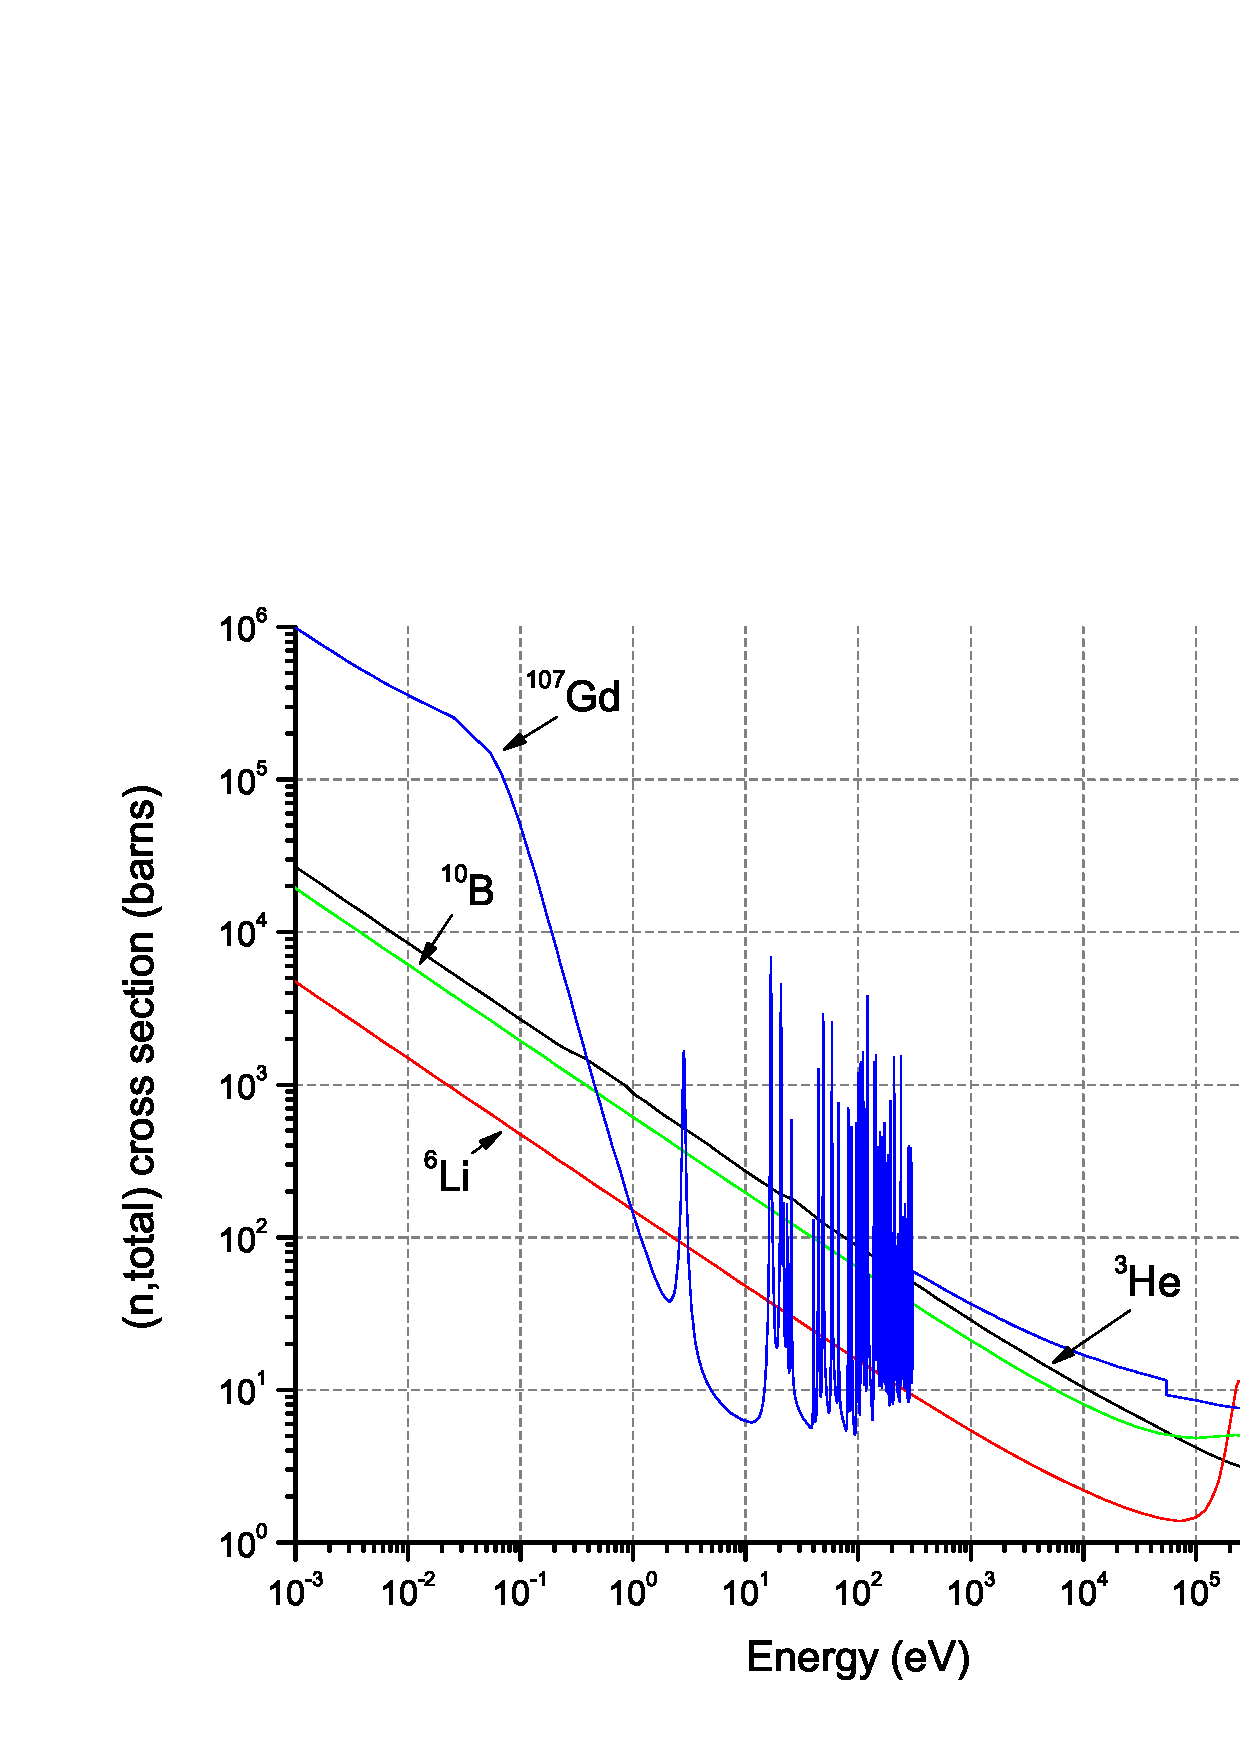
\includegraphics[width=\textwidth]{NeutronXS}
	\caption[Neutron Reaction Cross Sections]{Cross sections of typical isotopes used in neutron radiation detectors.  Neutrons at room temperature have an energy of \SI{0.025}{\eV}.}
	\label{fig:NeutronXS}
\end{figure}



%%%%%%%%%%%%%%%%%%%%%%%%%%%%%%%%%%%%%%%%%%%%%%%%%%%%%%%%%%%%%%%%%%%%%%%%%%%
%                                                                         %
%                      ENERGY SCALE AND RANGES                            %
%                                                                         %
%%%%%%%%%%%%%%%%%%%%%%%%%%%%%%%%%%%%%%%%%%%%%%%%%%%%%%%%%%%%%%%%%%%%%%%%%%%
\section{Charged Particle Interactions and Ranges}
\label{sec:InteractionsAndRange}
%%%%%%%%%%%%%%%%%%%%%%%%%%%%%%%%%%%%%%%%%%%%%%%%%%%%%%%%%%%%%%%%%%%%%%%%%%%
%                                                                         %
%                      ENERGY SCALE AND RANGES                            %
%                                                                         %
%%%%%%%%%%%%%%%%%%%%%%%%%%%%%%%%%%%%%%%%%%%%%%%%%%%%%%%%%%%%%%%%%%%%%%%%%%%
%% Simulation Caption Commands

% Content
The theoretical basis for the difference in energy deposition lies in the different mechanisms between charged particle interactions and photon interactions in matter.
For photons with energies between approximately \SI{0.5}{\MeV} and \SI{5}{\MeV} Compton scattering is the predominant interaction mechanism between the material and the photon.
The probability of an electron having a given kinetic energy after scattering can be expressed as \eqref{eqn:dSdEKleinNishina} (see \autoref{chap:ComptonScatter} for derivation details)
\begin{align}
  \label{eqn:dSdEKleinNishina}
\frac{d\sigma}{dE_e} = 2\pi r_e^2 \sin \theta f(\theta)\left [ \frac{1+\frac{E}{m_e c^2}\left(1-\cos\theta \right)^2}{E^2 \sin \theta} \right ]
\end{align}
provided  $f(\theta)$ is defined as $f(\theta) = \frac{1}{2}\left(\frac{E'}{E}\right)^2 \left(\frac{E'}{E} + \frac{E}{E'}-\sin^2\theta\right)$.
This distribution is shown for \iso[60]{Co} in \autoref{fig:Co60ComptonScatterSpectra}.
It is then highly likely that the Compton scattered electron will have an energy close to that of the maximum energy for the Compton scattering, \SI{0.96}{\MeV} for the \SI{1.173}{\MeV} photon and \SI{1.12}{\MeV} for the \SI{1.33}{\MeV} photon.
\begin{table}
	\caption[Characterstic Energies of Compton Scattered Electrons from Co-60]{Characteristic kinetic energies of the electrons from a Compton scattering of the two photons from \iso[60]{Co}. It is very likely that an electron will have a kinetic energy greater than \SI{0.8}{\MeV}, which has a range of \SI{0.34}{\gram\per\cm\squared} in polystyrene}.
	\label{tab:ComptonEnergiesCo60}
	\begin{tabular}{ m{4cm} m{3cm} m{3cm} m{3cm}}
	\toprule
	Gamma Energy & Mean Electron Energy & Median Electron Energy & Maximum Electron Energy \\
	\midrule
	\SI{1.17}{\MeV} & \SI{0.68}{\MeV} & \SI{0.82}{\MeV} & \SI{0.96}{\MeV} \\
	\SI{1.33}{\MeV} & \SI{0.80}{\MeV} & \SI{0.96}{\MeV} & \SI{1.12}{\MeV} \\
	Average & \SI{0.74}{\MeV} & \SI{0.89}{\MeV} &  \\
	\bottomrule
	\end{tabular}
\end{table}
\begin{figure}
  \centering
    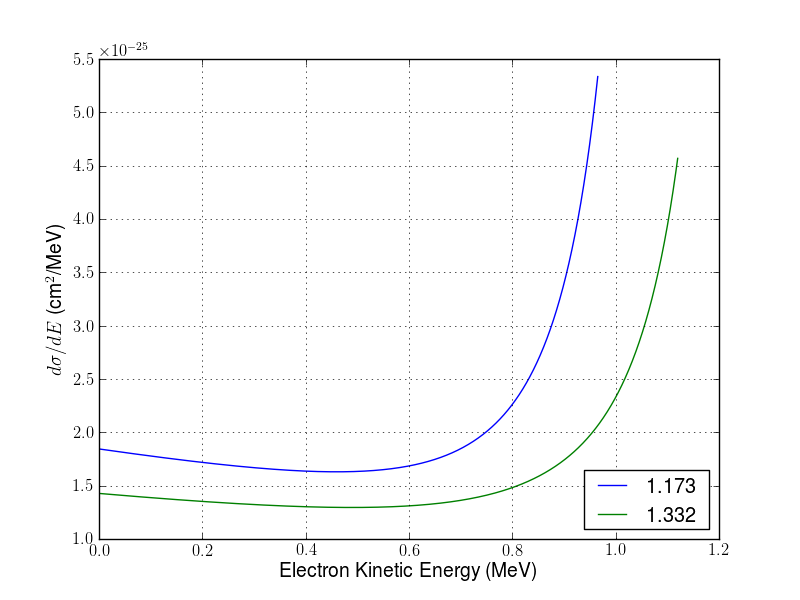
\includegraphics[width=\textwidth]{Co60ComptonScatteredSpectra}
    \caption[Analytical Co-60 Compton Electron Differential Microscopic Cross Section]{Co-60 Compton Electron Differential Microscopic Cross Section. The relative probabilities of a Compton Scattered Electron having a given kinetic energy from \iso[60]{Co} can be determined by their relative differential microscopic cross sections. For example, it almost two and a half times more likely that a Compton scattered electron will have a kinetic energy of \SI{0.95}{\MeV} than \SI{0.75}{\MeV}.}
    \label{fig:Co60ComptonScatterSpectra}
  \end{figure}
\begin{figure}
    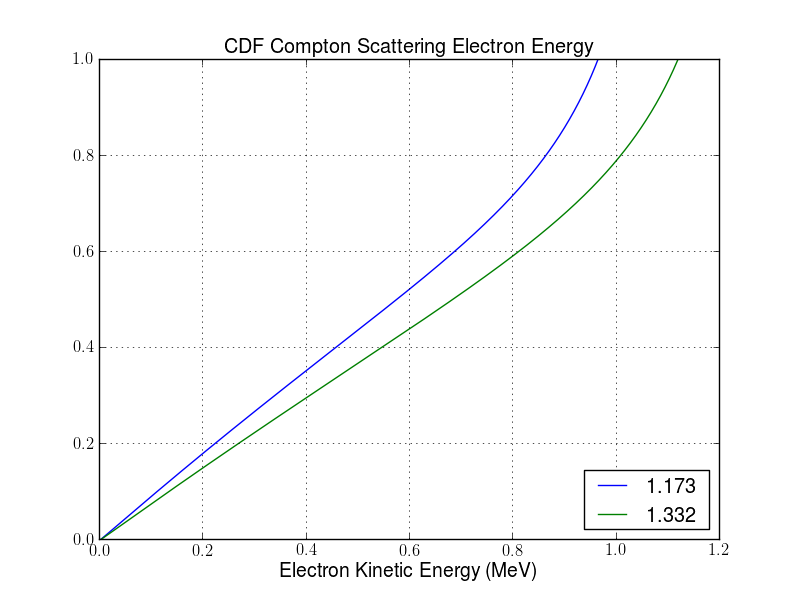
\includegraphics[width=\textwidth]{Co60ComptonScatteredSpectraCDF}
    \caption[Analytical Co-60 Compton Electron Kinetic Energy Cumulative Distribution]{Probability of the energy of a Compton Scattered Electron from \iso[60]{Co}. Over half of the electrons from the Compton scattering will have an energy greater than \SI{0.5}{\MeV}}
    \label{fig:Co60ComptonScatterCDF}
\end{figure}
The cumulative distribution function (CDF) is shown in \autoref{fig:Co60ComptonScatterCDF}.
In the case of $\iso[6]{Li}\left(n,\iso[3]{H}\right)\alpha$ the fission energy is distributed between a triton of energy \SI{2.73}{\mega\eV} and an alpha of energy \SI{2.05}{\mega\eV}.
The maximum kinetic energy of an electron from a Compton scattering event with an impingement \iso[60]{Co} source is \SI{1.117}{\mega\eV} (for the \SI{1.332}{\mega\eV} gamma). 
In polystyrene with a density of \SI{1}{\gram\per\cm\cubed}, the range of the maximum electron from Compton scattering is around \SI{4.5E3}{\um}\cite{berger_estar_2005}.
If elastic scattering between the alpha, triton and electrons is assumed the maximum kinetic energy of an electron is \SI{1.097}{\kilo\eV} for the alpha particle and \SI{1.986}{\kilo\eV} for the triton\cite{turner_atoms_2008}.
The range of the electron from a gamma interaction is more than \num{1E3} times greater than the range of electrons from an alpha or triton (\autoref{tab:BasicEDepOutline}).
Therefore, it is more likely that the electrons generated by the alpha and the triton deposit significantly more of their energy in a thin film than the electron from a gamma.
This is also reflected in the stopping power, where the reaction product secondary electrons have a stopping power 40 times that of the secondary electrons from a gamma \cite{berger_estar_2005}.
The simulated electron range distributions for several energies is shown in \autoref{fig:ElectronRangesDist} and summarized in \autoref{fig:ElectronRanges}.
The electrons  from Compton scattering of \iso[60]{Co} will be on the order of \SI{100}{\keV} , with ranges two orders of magnitude than that of electrons from the charged particle interactions.
\begin{table}[ht]
  \caption[Electron Energy, Range, and Stopping Power]{Electron Energy, Range, and Stopping Power \protect\cite{berger_estar_2005,turner_atoms_2008}}
	\centering
	\begin{tabular}{c | c S c}
	\toprule
	{Electron Parent} & {Electron Energy} & {Total Stopping Power} & {CSDA Range} \\
	 &  & \si{\mega\eV \cm\squared \per \gram} & \si{\gram\per\cm\squared} \\
	\midrule
	{gamma}  & \SI{1.12}{\mega\eV} & 1.79 & $\ge$~\num{4.48E-1} \\
	{triton} & \SI{1.99}{\kilo\eV} & 75.1 & $\le$~\num{2.55E-4} \\
	{alpha}  & \SI{1.10}{\kilo\eV} & 113  & $\le$~\num{2.55E-4} \\
	\bottomrule
	\end{tabular}
  \label{tab:BasicEDepOutline}
	% See pg. 87 of Matthew's lab notebook for the calculation
\end{table}
\begin{figure}
  \centering
      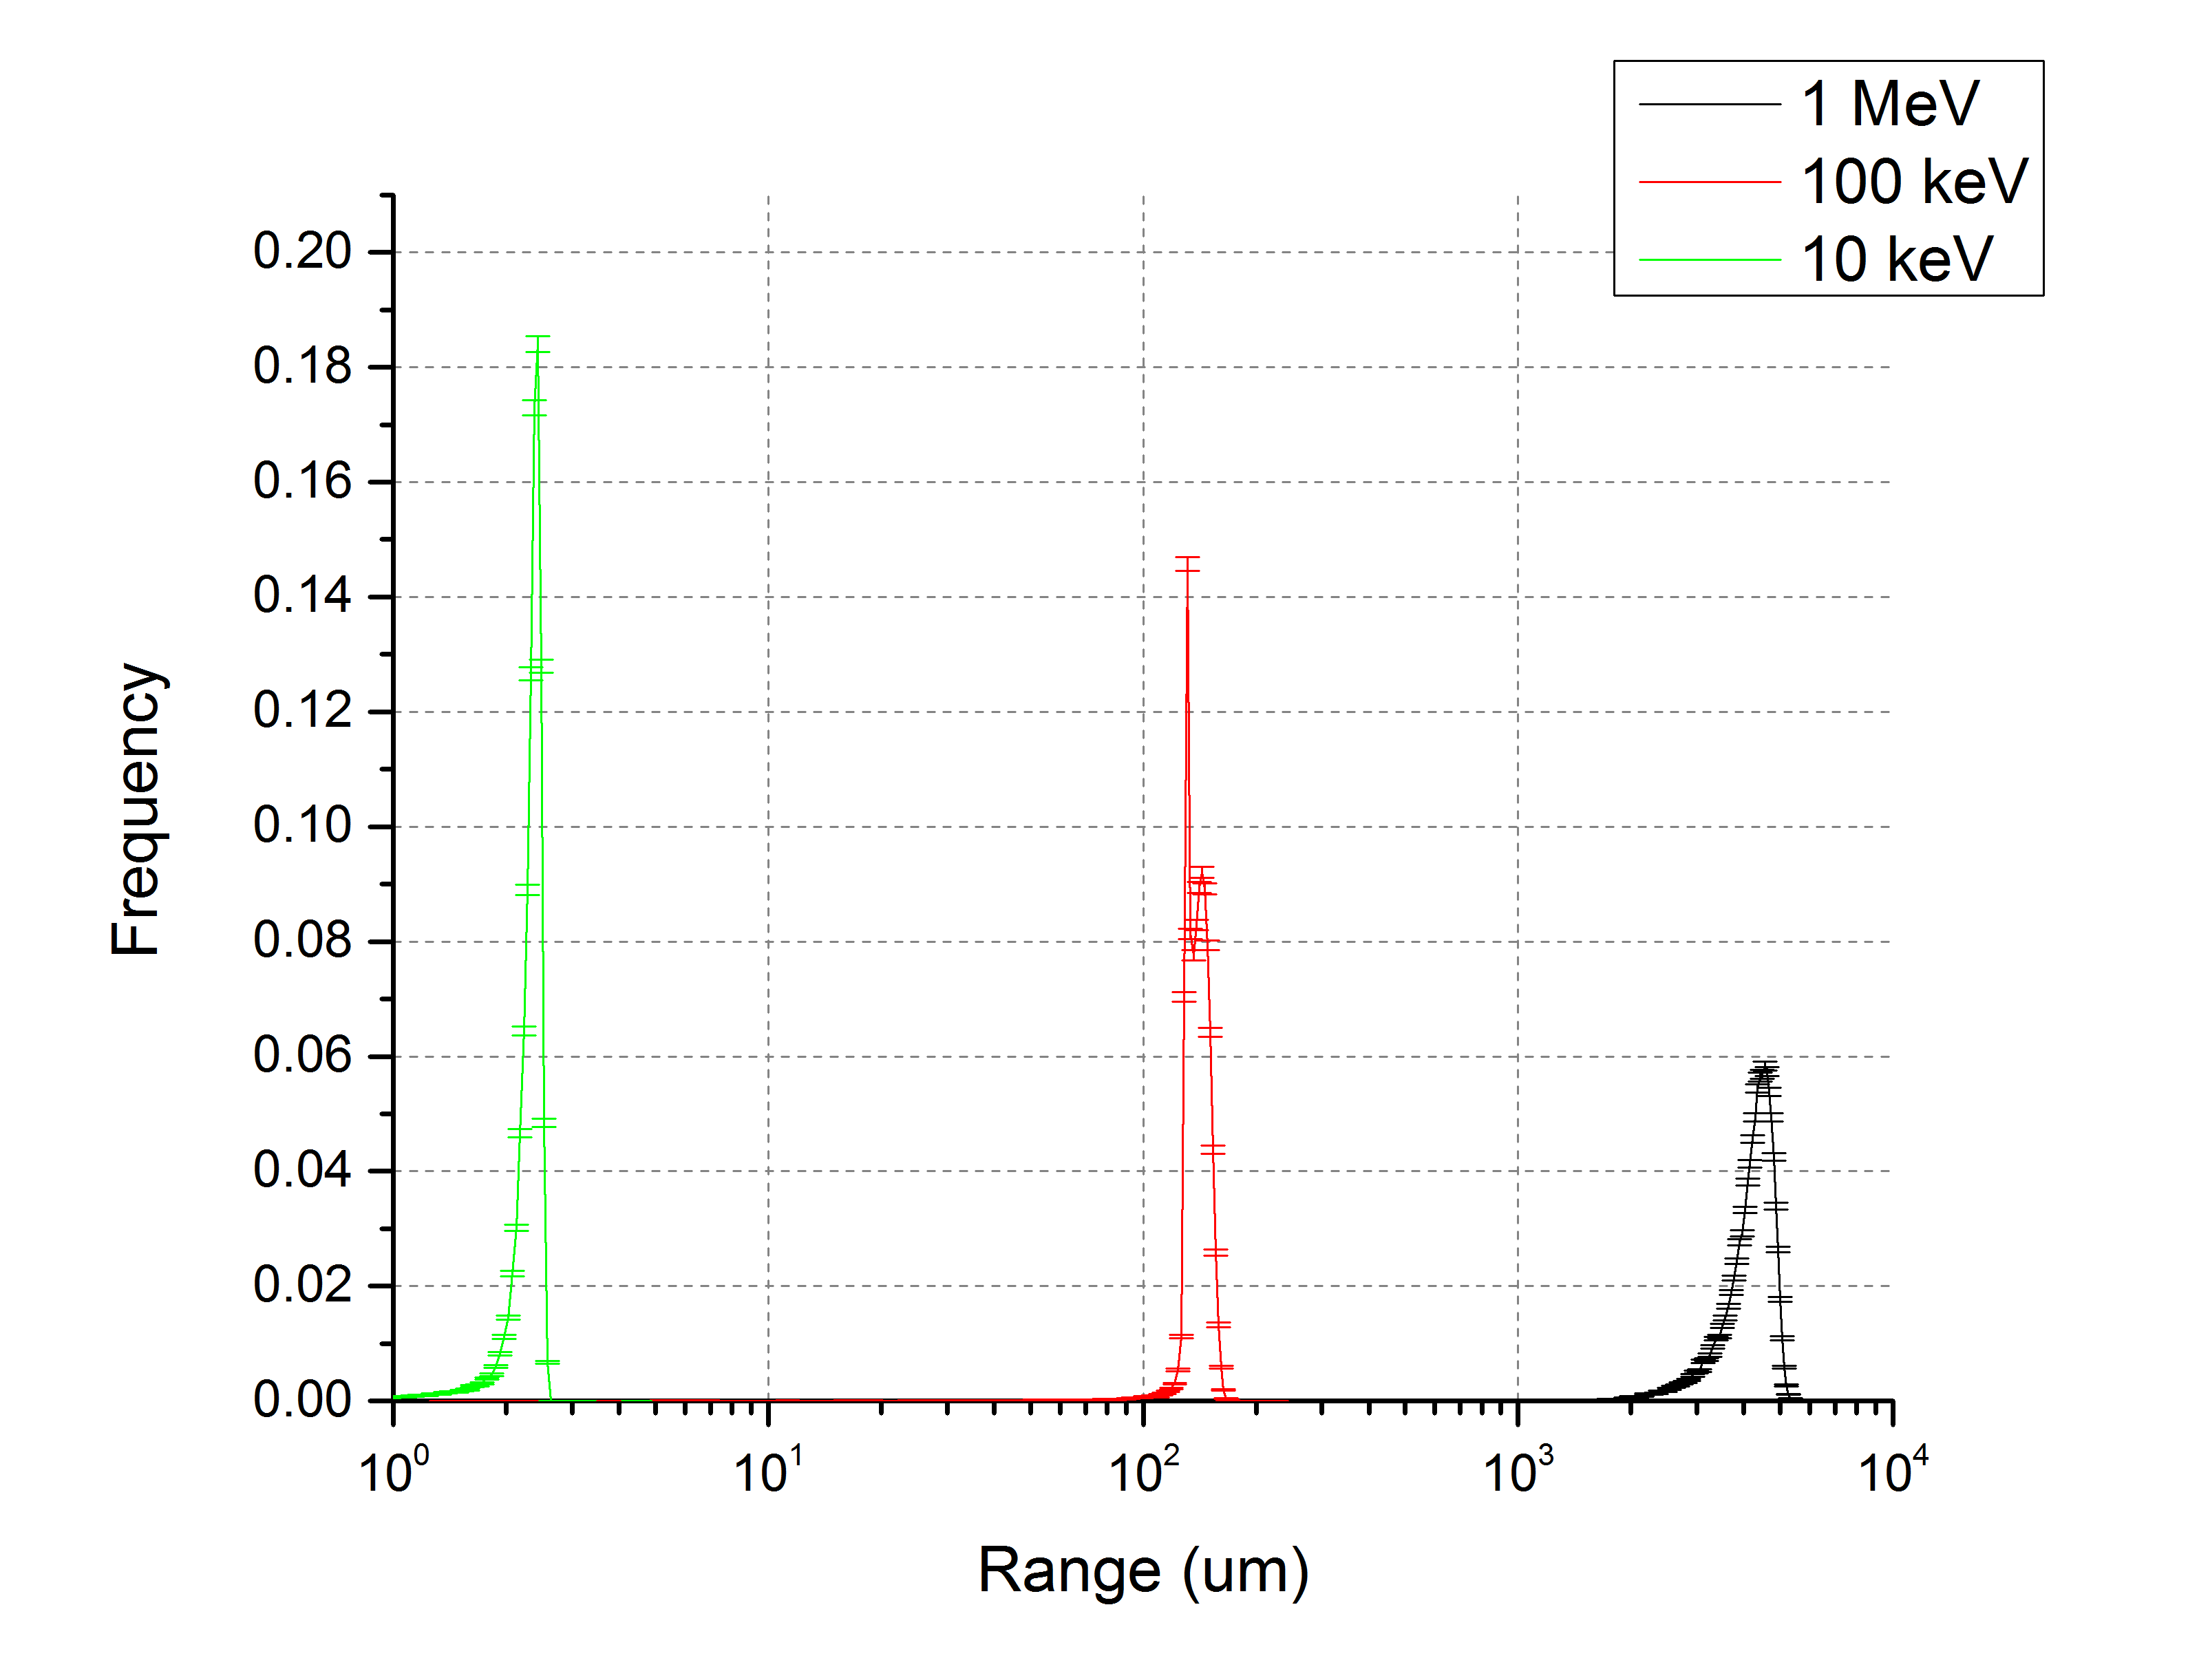
\includegraphics[width=\textwidth]{ElectronRangeDistribution}
      \caption[Simulated Electron Ranges Distrubtions in Polystyrene]{Simulated range of \SI{1}{\MeV}, \SI{100}{\keV}, and \SI{10}{\keV} electrons.\rangeSimGeo}
      \label{fig:ElectronRangesDist}
\end{figure}
\begin{figure}
	\centering
      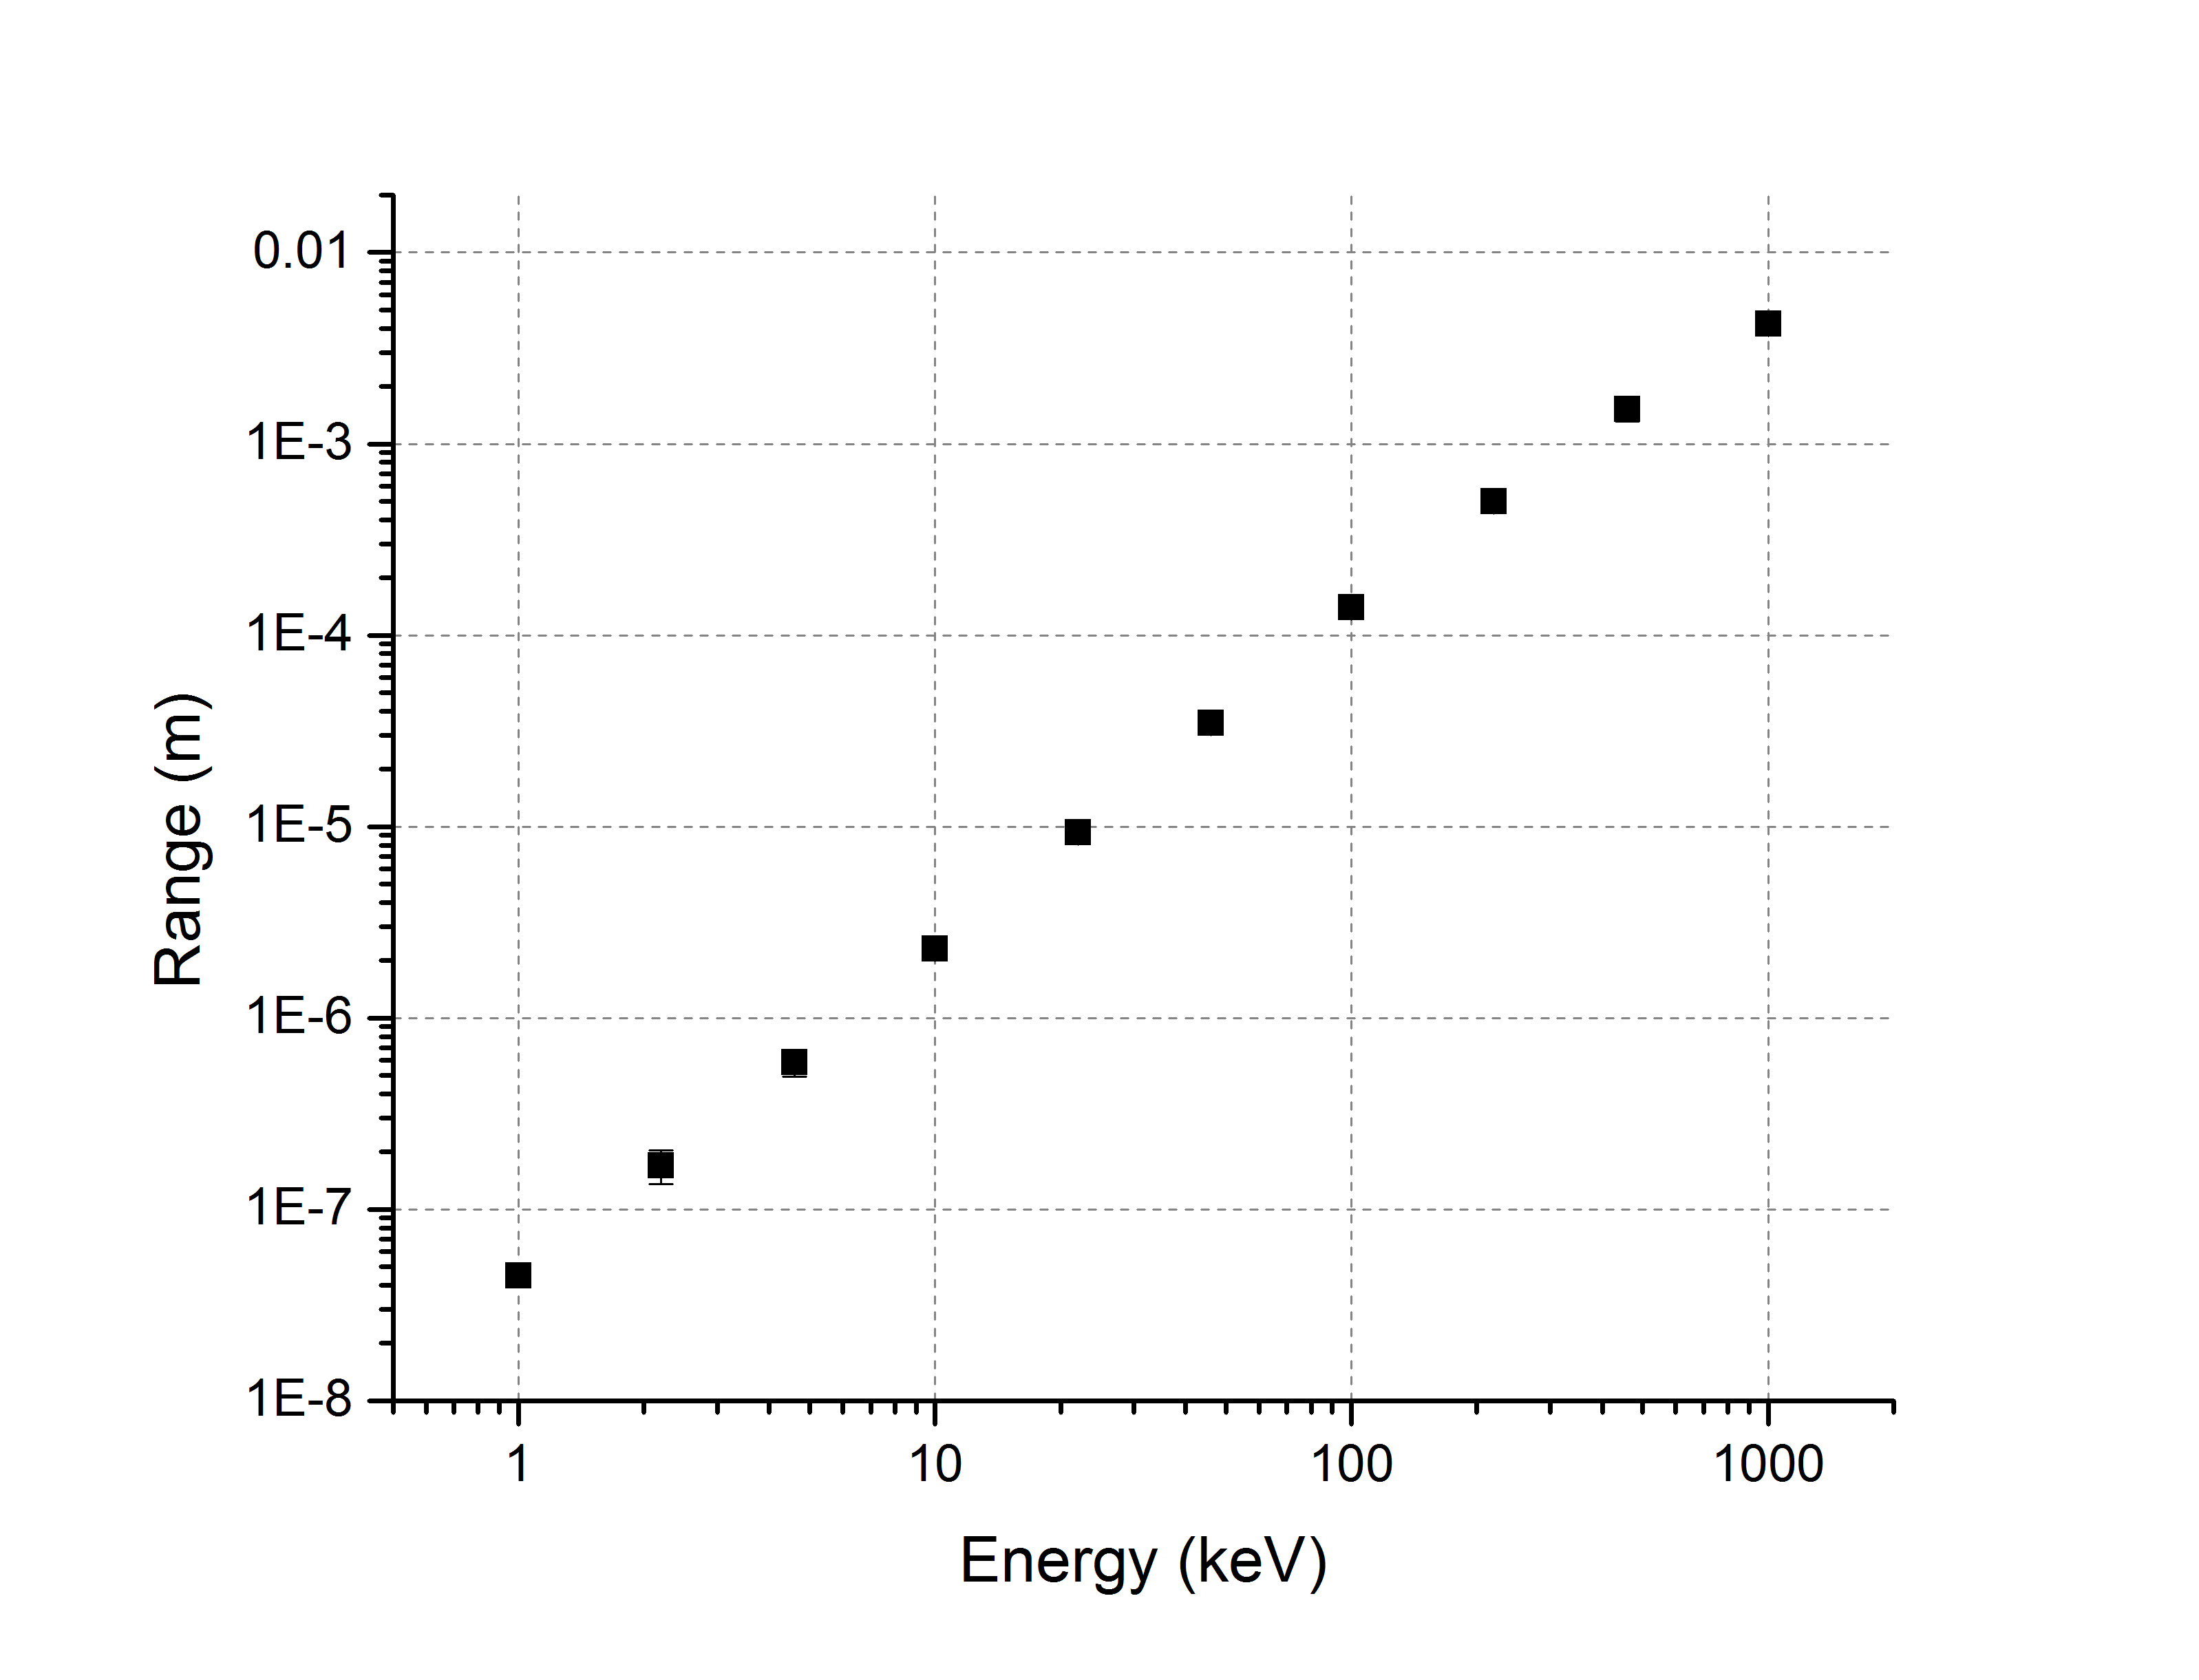
\includegraphics[width=\textwidth]{ElectronRange}
  \caption[Simulated Electron Ranges in Polystyrene]{Simulated electron ranges for electron kinetic energies ranging from \SI{1}{\keV} to \SI{1}{\MeV}.\rangeSimGeo} 
  \label{fig:ElectronRanges}
\end{figure}

The development of the secondary electron energy ranges so far has been from a simplified treatment of the problem when only the dominant process are considered.
Detailed simulations are necessary in order to have a greater understanding of the problem. 
The energy of the electrons created from an alpha (\SI{2.05}{\MeV}), triton (\SI{2.73}{\MeV}), and gammas from \iso[60]{Co} were calculated using a GEANT4 simulation, and overlaid on the range of electrons (left axis) as shown in \autoref{fig:ERangeAndDist}.
It is then clear that the electrons from the \iso[60]{Co} will travel much father than those from the $\iso[6]{Li}\left(n,\alpha\right)\iso[3]{H}$ reaction products.
\begin{figure}
  \centering
  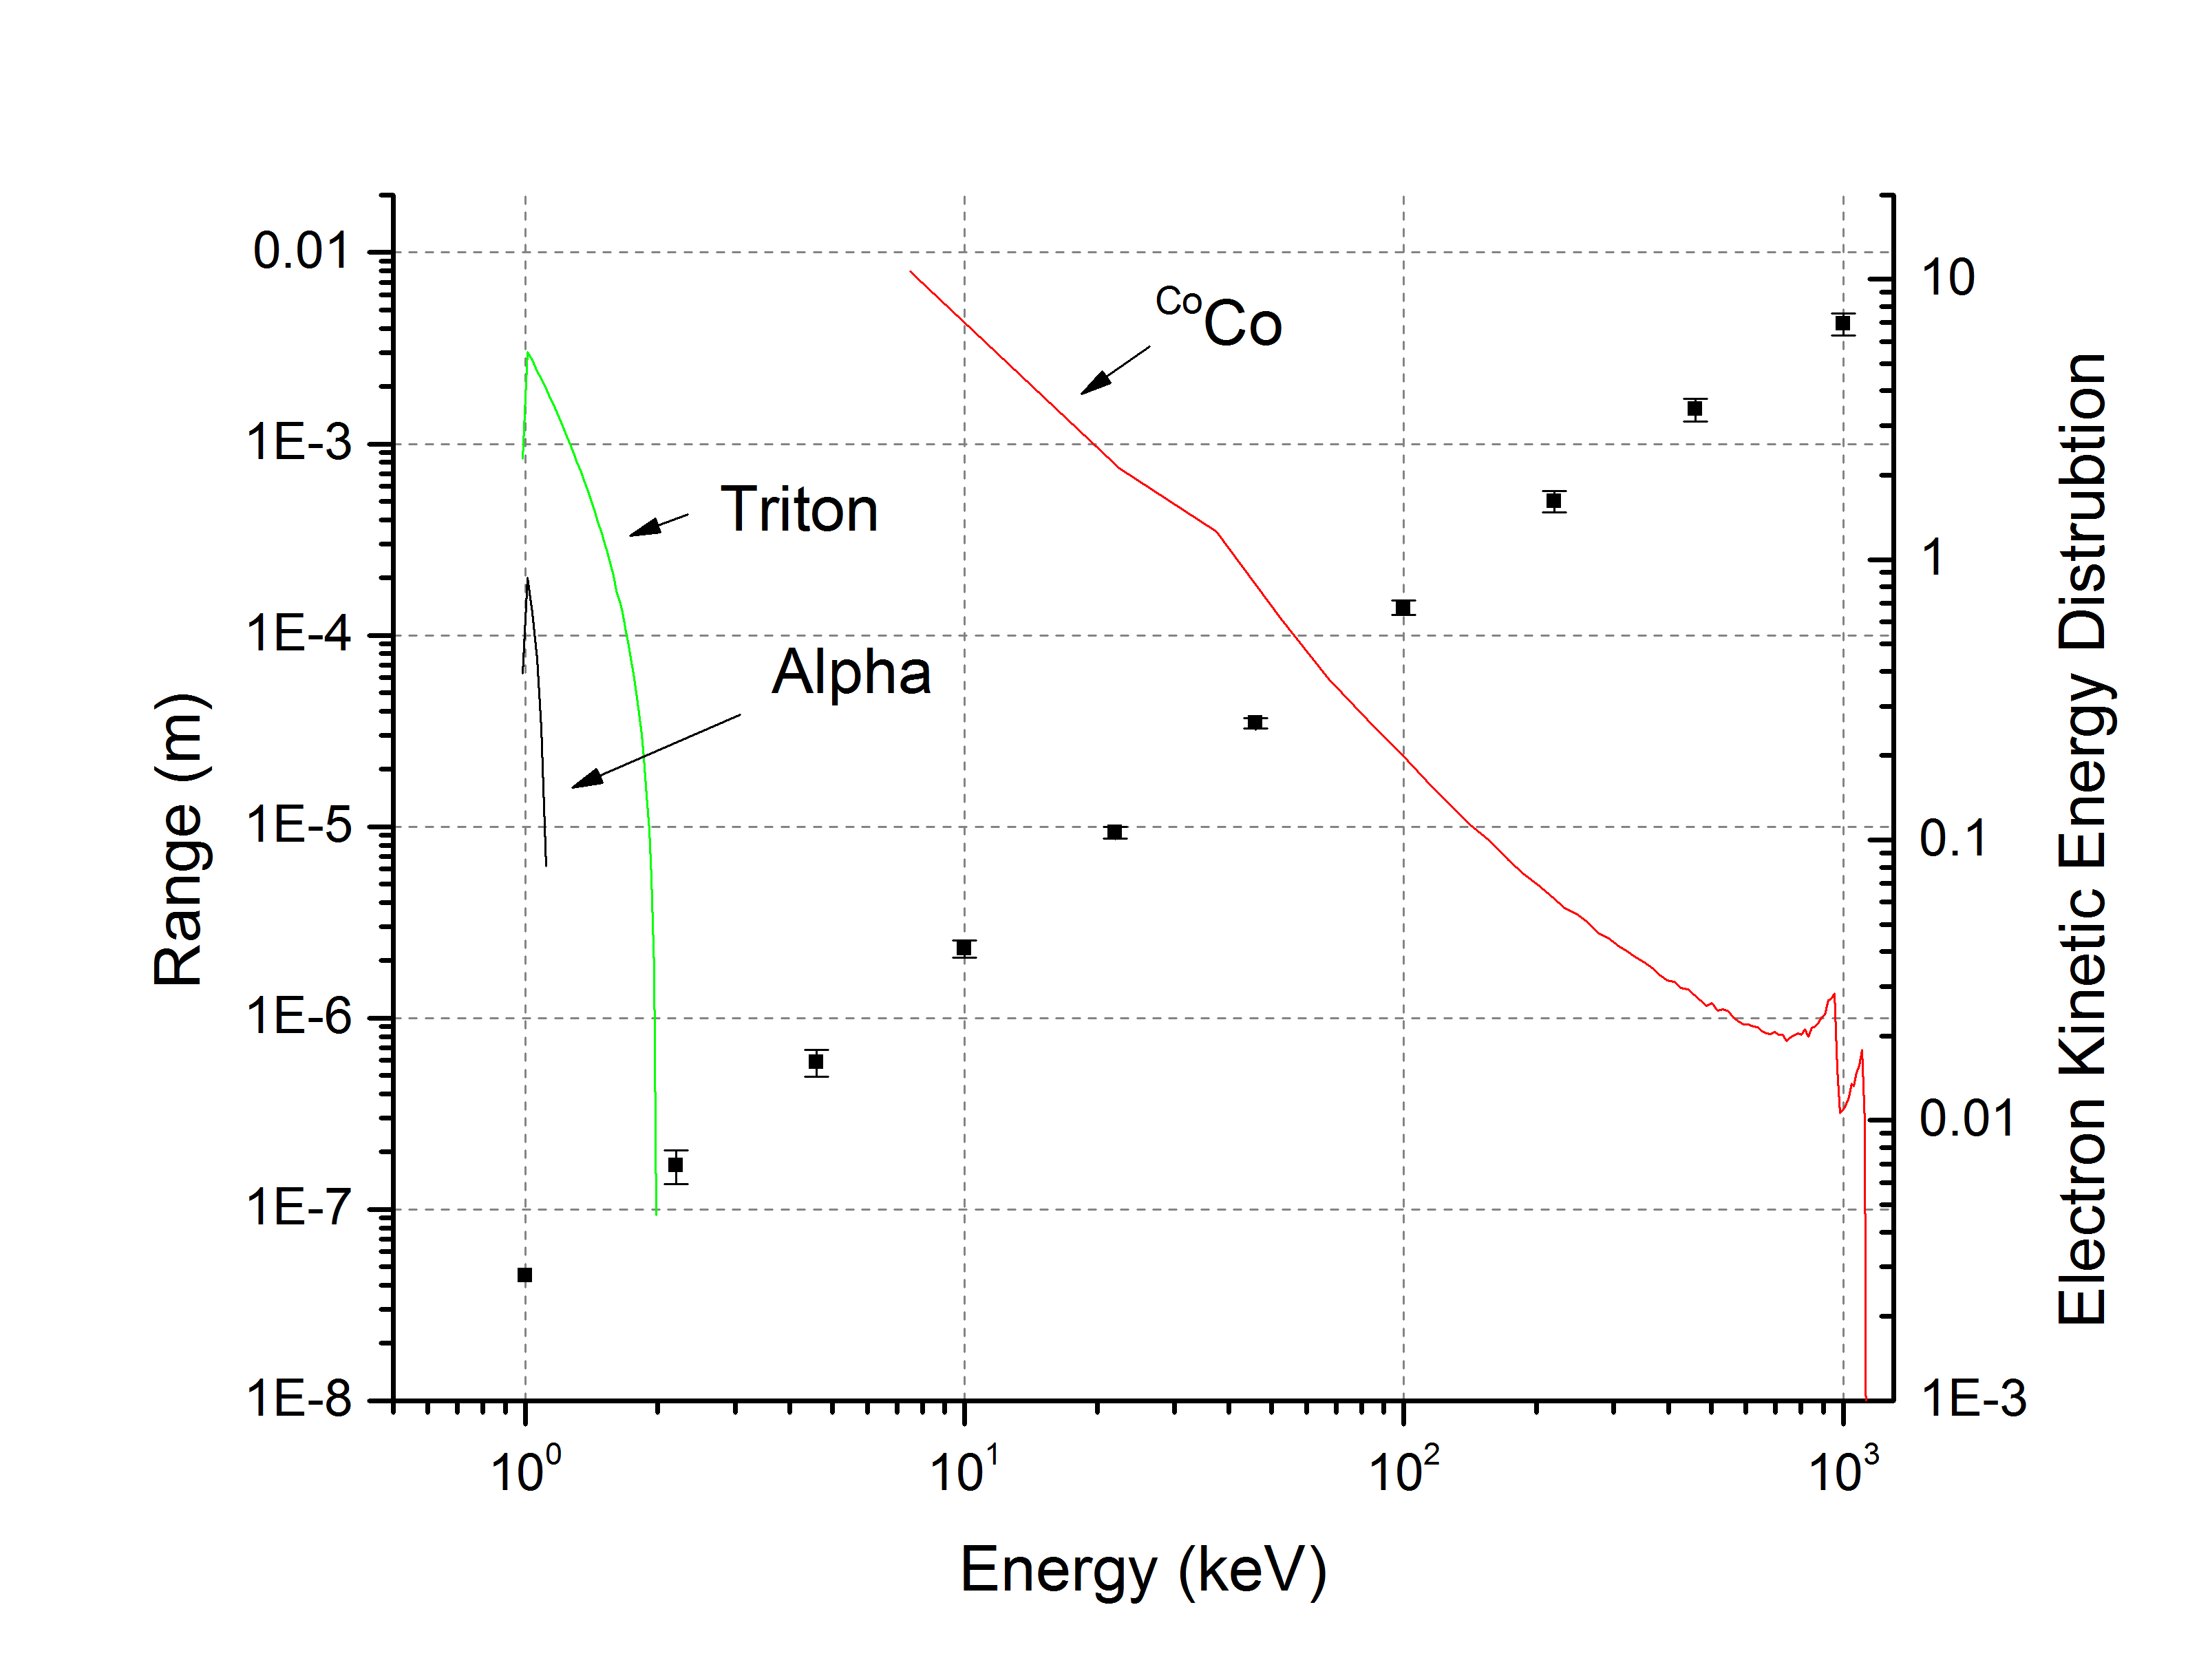
\includegraphics[width=\textwidth]{ElectronRangeAndEnergyDist}
  \caption[Electron Range and Energy Distribution of Selected Reactions]{The electron range (left axis) corresponding to the square dots overlaid with the kinetic energy of electrons from \SI{2.05}{\MeV} alpha, \SI{2.73}{\MeV} triton, and secondary electrons from \iso[60]{Co}. The \iso[60]{Co} electrons have energies much greater than the alpha and triton, and their corresponding range is orders of magnitude greater than the ranges of the electrons from the alpha and triton. \rangeSimGeo}
  \label{fig:ERangeAndDist}
\end{figure}


%%%%%%%%%%%%%%%%%%%%%%%%%%%%%%%%%%%%%%%%%%%%%%%%%%%%%%%%%%%%%%%%%%%%%%%%%%%
%                                                                         %
%                      SCINTILLATION MECHANICS                            %
%                                                                         %
%%%%%%%%%%%%%%%%%%%%%%%%%%%%%%%%%%%%%%%%%%%%%%%%%%%%%%%%%%%%%%%%%%%%%%%%%%%
\section{Scintillation Mechanisms}
\label{sec:ScintMechanics}
%%%%%%%%%%%%%%%%%%%%%%%%%%%%%%%%%%%%%%%%%%%%%%%%%%%%%%%%%%%%%%%%%%%%%%%%%%%
%                                                                         %
%                         Introduction to Scintillation                   %
%                                                                         %
%%%%%%%%%%%%%%%%%%%%%%%%%%%%%%%%%%%%%%%%%%%%%%%%%%%%%%%%%%%%%%%%%%%%%%%%%%%
Scintillation detectors (the detectors on which this work is based) utilize a scintillator to convert ionizing radiation into photons, and then transporting and capturing those the emitted photons, commonly with a photomultiplier tube (PMT).
The electrical signal from the PMT is then an indicator of a radiation event in the detector's scintillator material.
The current RPMs with \iso[3]{He} are ion chamber detectors, however, the proposed \iso[6]{Li} glass detectors and \iso[6]{LiF} doped ZnS:Ag detectors are scintillation based detectors. 

\subsection{Organic Scintillators}
An organic scintillator generally has a $\pi$-electron structure similar to that of \autoref{fig:benzePiStructure} with typical energy levels as shown in \autoref{fig:pielectron}.
An incoming electron (liberated from the energy deposition of the ionizing radiation) then excites one of the modes of the $\pi$-electron structure.
Higher singlet states rapidly (on the order of picoseconds) relax to the first singlet state, and excessive vibrational energy (populations of the vibrational sates) is lost.
Thus, after a short period of time the entire excitation population is in the $S_10$ state, and the decay of this state creates the prompt fluorescence.
\begin{figure}
	\centering
	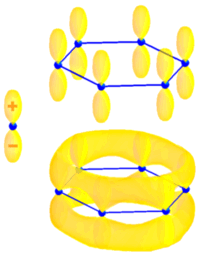
\includegraphics[width=0.5\textwidth]{benzeneStructure}
	\caption[Example orbitals for Benzene]{Example electron orbitals for Benzene.  The distributed, non-localized electron structure of the bottom image is typically of that of scintillators.}
	\label{fig:benzePiStructure}
\end{figure}
\begin{figure}
  \centering
  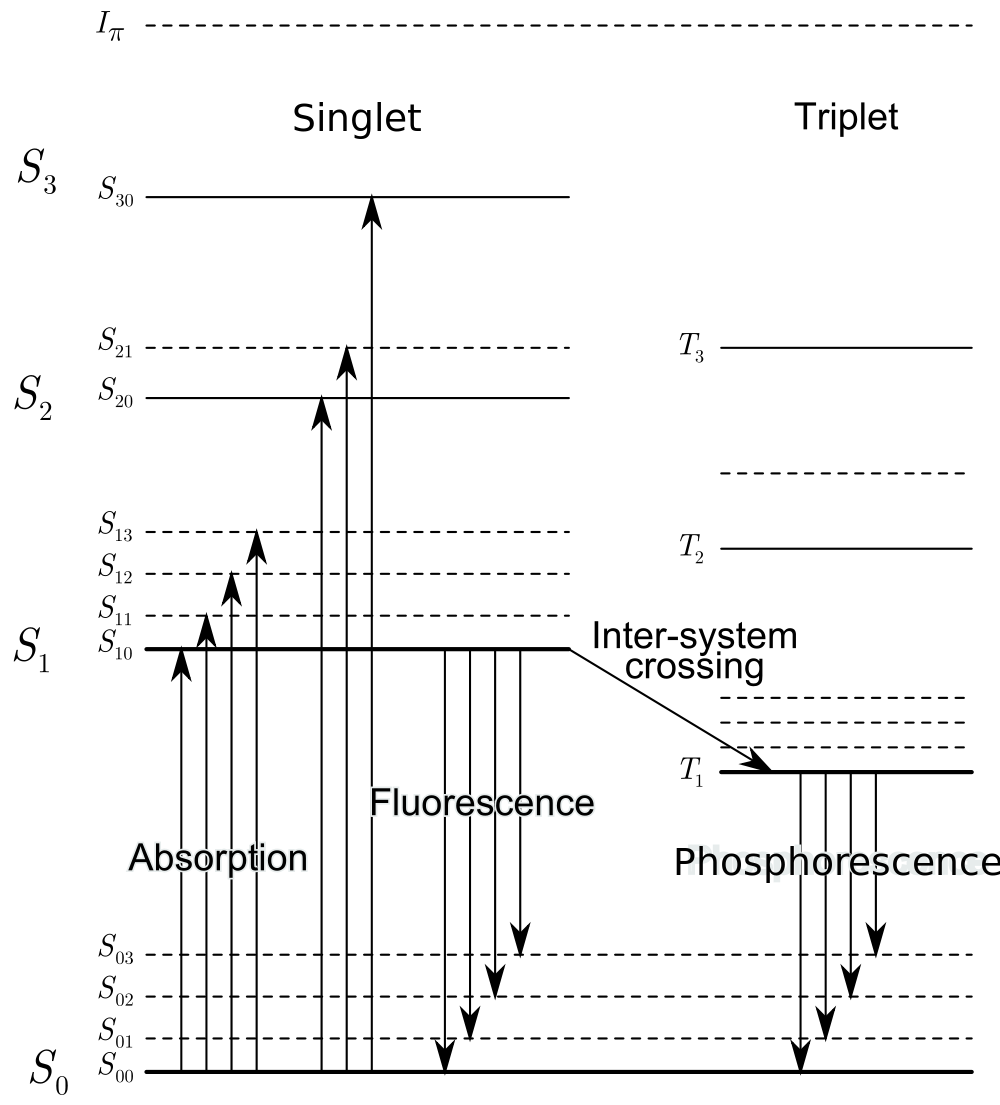
\includegraphics[width=0.6\textwidth]{PiElectronSates}
  \caption[$\pi$ Electron Structure]{Typical $\pi$-electron structure of an organic molecule. The ground state of the molecule is shown as $S_0$, and excited single states are $S_1$, $S_2$ etc The triplet states are $T_1$, $T_2$, with the vibrational states as $S_OO$, $S_01$, $S_02$ and so forth. Figure from Wikipedia.}
  \label{fig:pielectron}
\end{figure}
The excitations of triplet states typically yield delayed scintillation events or phosphorescence.
An excited triplet states immediately decays to the $T_0$ state by internal degradation without a photon emission.
The $T_0$ state typically decays by interacting with another $T_0$ state in a $T_0 + T_0 \to S^* + S_0 + h\nu$ transition.
The excited singlet state $S^*$ then also decays to the $S_0$ state.
The $T_0 + T_0$ transitions is slower than direct singlet state de-excitations, and results in a slow component of the pulse, which can be used for pulse shape discrimination.

The light output of an organic scintillator can be empirically related to the energy deposition in the scintillator through the Birks equation.
In the absence of any quenching it is assumed that the light output per unit length is directly proportional to the energy deposition per unit length \eqref{eqn:LONoQuench}
\begin{align}
  \label{eqn:LONoQuench}
    \frac{dL}{dx} = S_B\frac{dE}{dx}
\end{align}
where \definevar{$S_B$}{absolute scintillation efficiency} and \definevar{$\frac{dE}{dx}$}{linear stopping power} .
If quenching of the light from molecules damaged by the radiation is also assumed to be proportional to the energy deposition per track length, than the Birks equation can be written as \eqref{eqn:BirksEquation}
\begin{align}
  \label{eqn:BirksEquation}
    \frac{dL}{dx} = \frac{S_B\frac{dE}{dx}}{1+kB\frac{dE}{dx}}
    \end{align}
    where \definevar{$kB$}{Birks parameter} which accounts for the quenching of the light.
For low stopping powers (or particles with a very high energy) the light output per unit track length is linear as the quenching term can be neglected.
However, for particles with a large stopping power the light output along the track length becomes saturated by quenching.
This difference in the pulse height accounts for that difference in light output from a \SI{1}{\MeV} electron compared to a \SI{1}{\MeV} alpha.
The \textit{alpha to beta} ratio provides a measure of this effect, and for the GS20 glass is it typically around 0.23.
This effect is critical in the developed detectors are the reaction products of of the \iso[6]{Li} neutron absorption are both heavily charged particles subject to this effect.
Thus, while there is \SI{4.78}{\MeV} of reaction product energy released in the neutron absorption, the low alpha to beta ratio of the material limits the actual number of scintillation events.

\subsection{Pulse Height Deficit}
The concept of alpha to beta ratio is extended for other charged ions as the pulse height deficit.
The pulse height deficit is defined as a measure the apparent energy loss (as seen from the pulse height) of a heavy charged ion compared to an electron.  
The apparent loss in energy of the heavy charged charged ions relative to
This is measured as the difference between the energy of the heavy ion and its apparent energy from the pulse height.  
Several researchers have investigated the light output of scintillators in response to different types of ionizing radiation.
\autoref{fig:lightYieldVerbinski} summarizes the results of \cite{Verbinski_1968} in which the pulse height deficit is apparent for the as the charged ions become heavier.
\begin{figure}
  \centering
  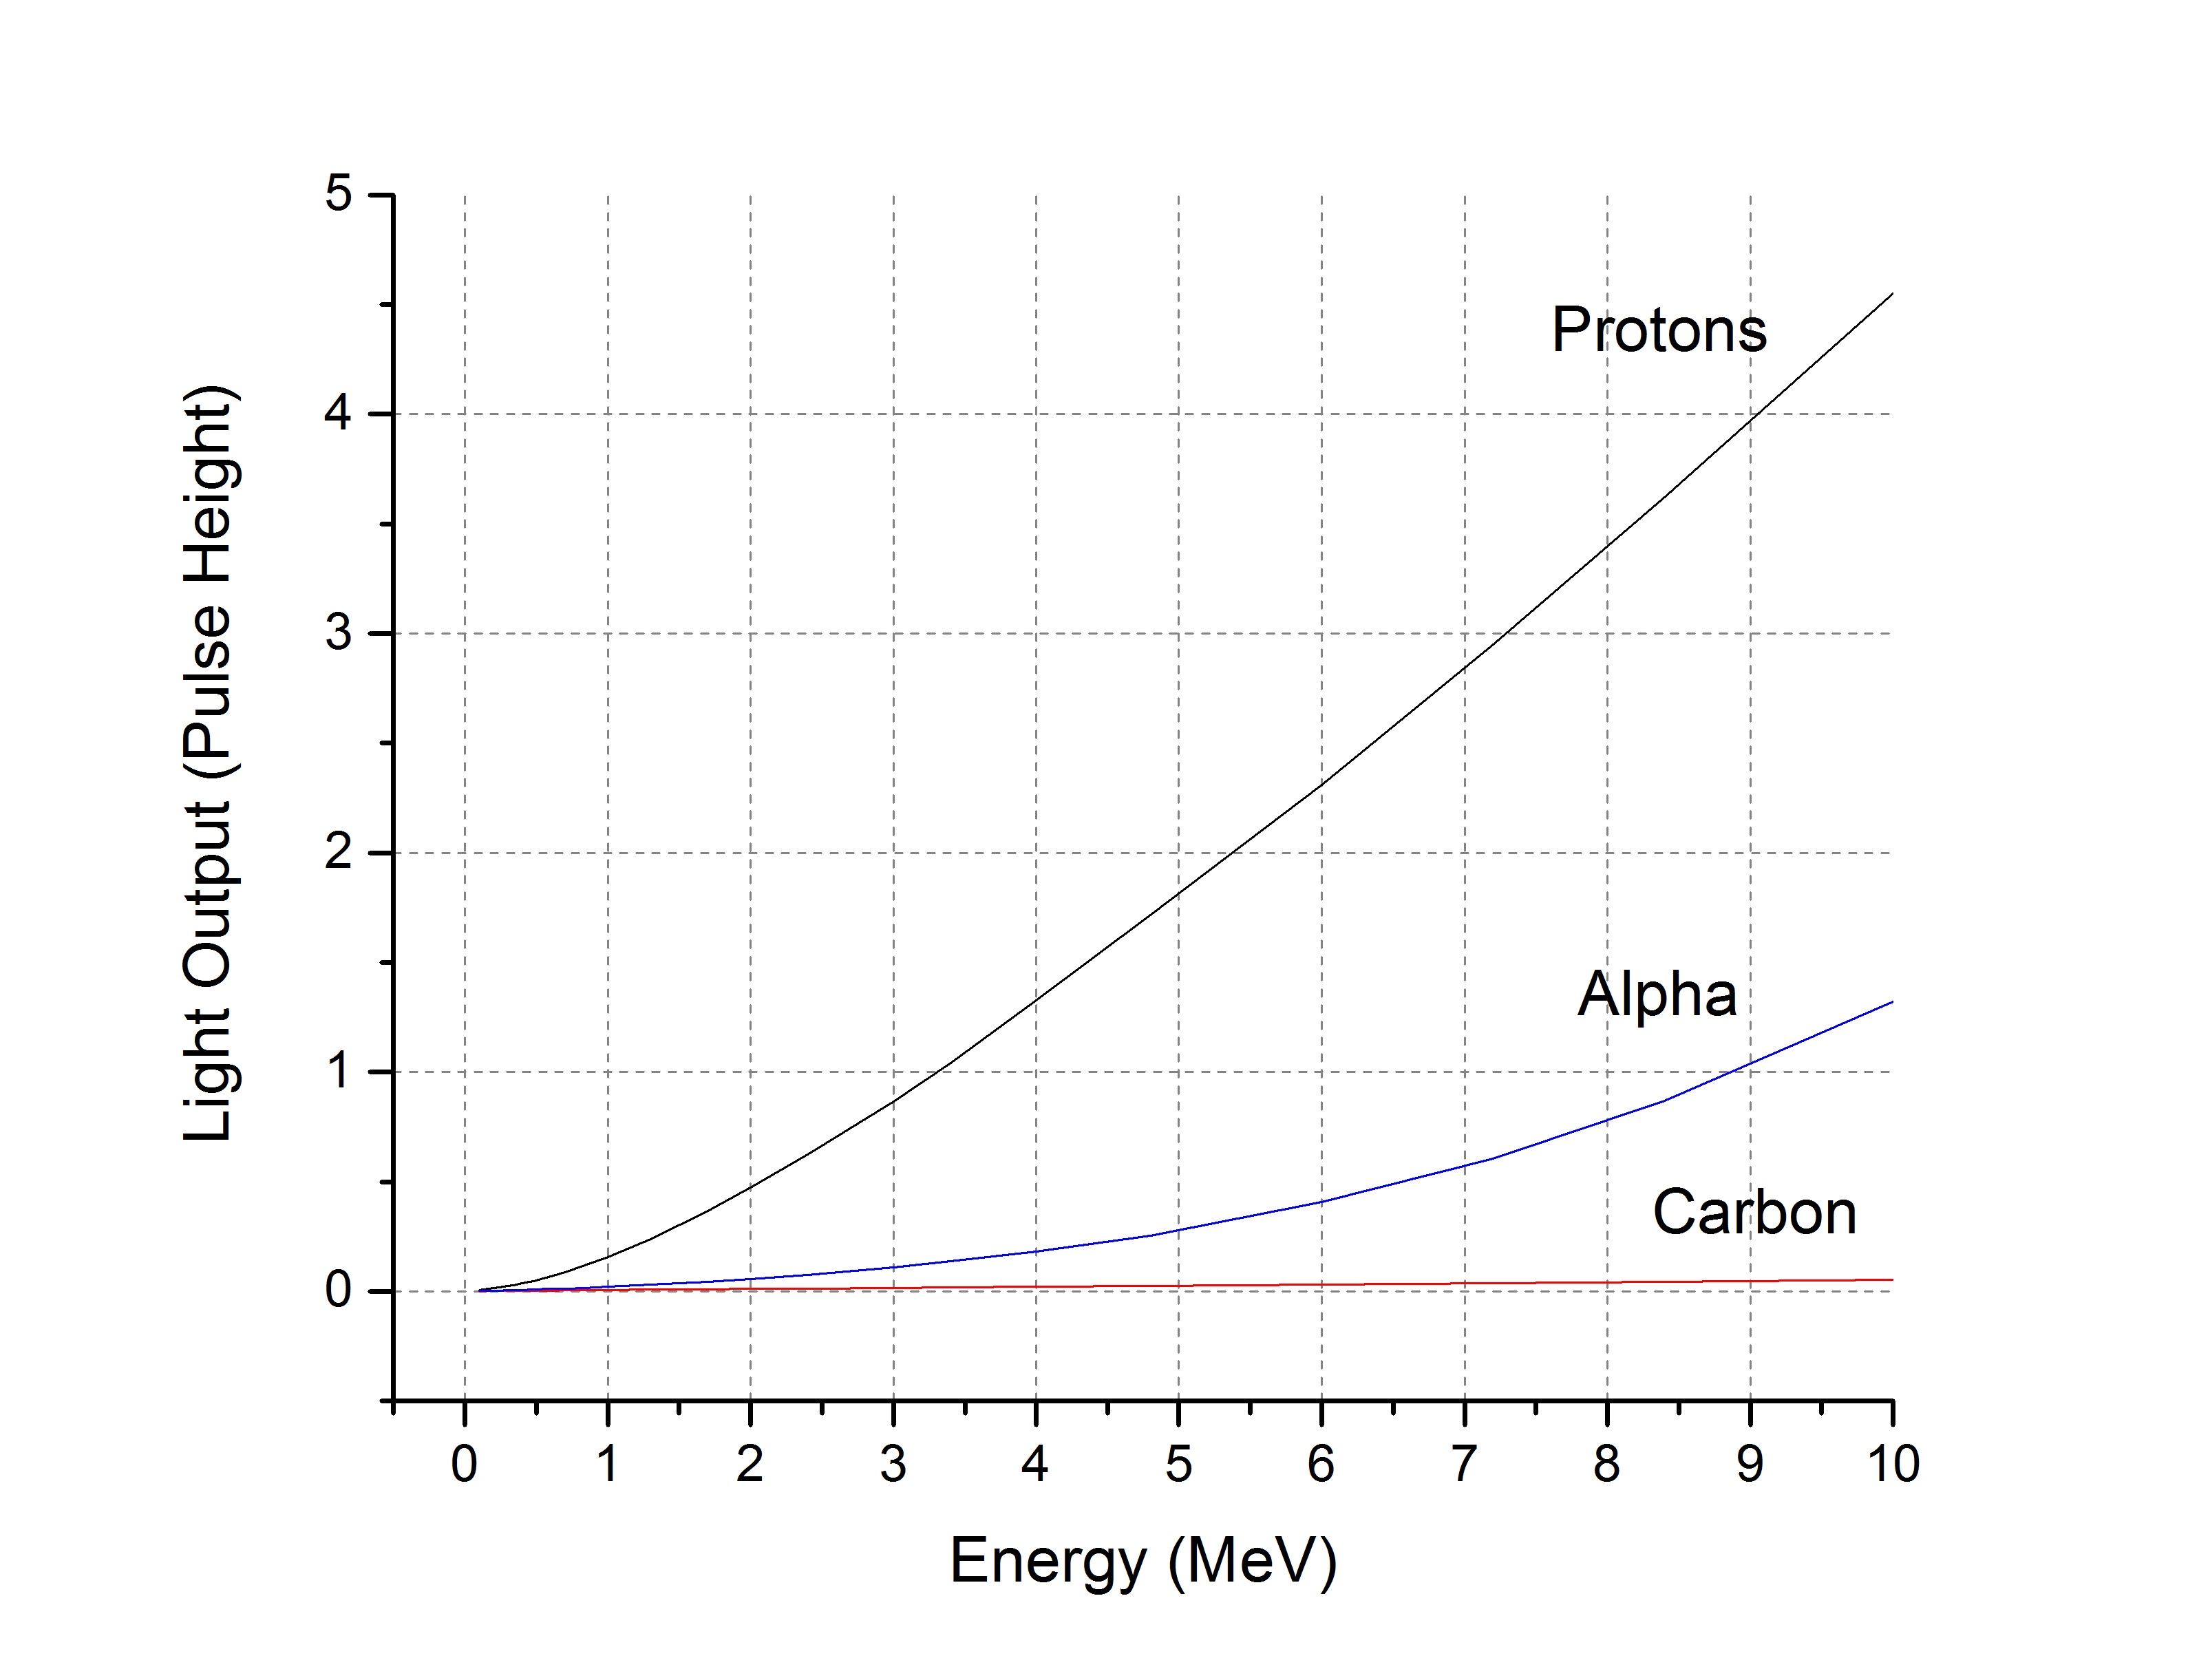
\includegraphics[width=\textwidth]{Verbinski_LightYield_AlpahCarbonProton}
  \caption[Light yield non-proporitonality of anthracene]{Light yield non-proproitonality of anthracene. Data from \cite{Verbinski_1968}.}
  \label{fig:lightYieldVerbinski}
\end{figure}

An illustration of the energy deposition between the different particles resulting in the pulse height deficit is presented in \autoref{fig:ParticleTracks}.
The electrons, with their low stopping power and broad track structure deposit their energy over a broader range than do the heavy charged ions (which tend to have rather collimated tracks).
Thus, the heavy charged ions deposit a large amount of their energy in a small volume, completely ionizing that volume and inhibiting scintillation.
\begin{figure}
  \begin{subfigure}[b]{0.45\textwidth}
    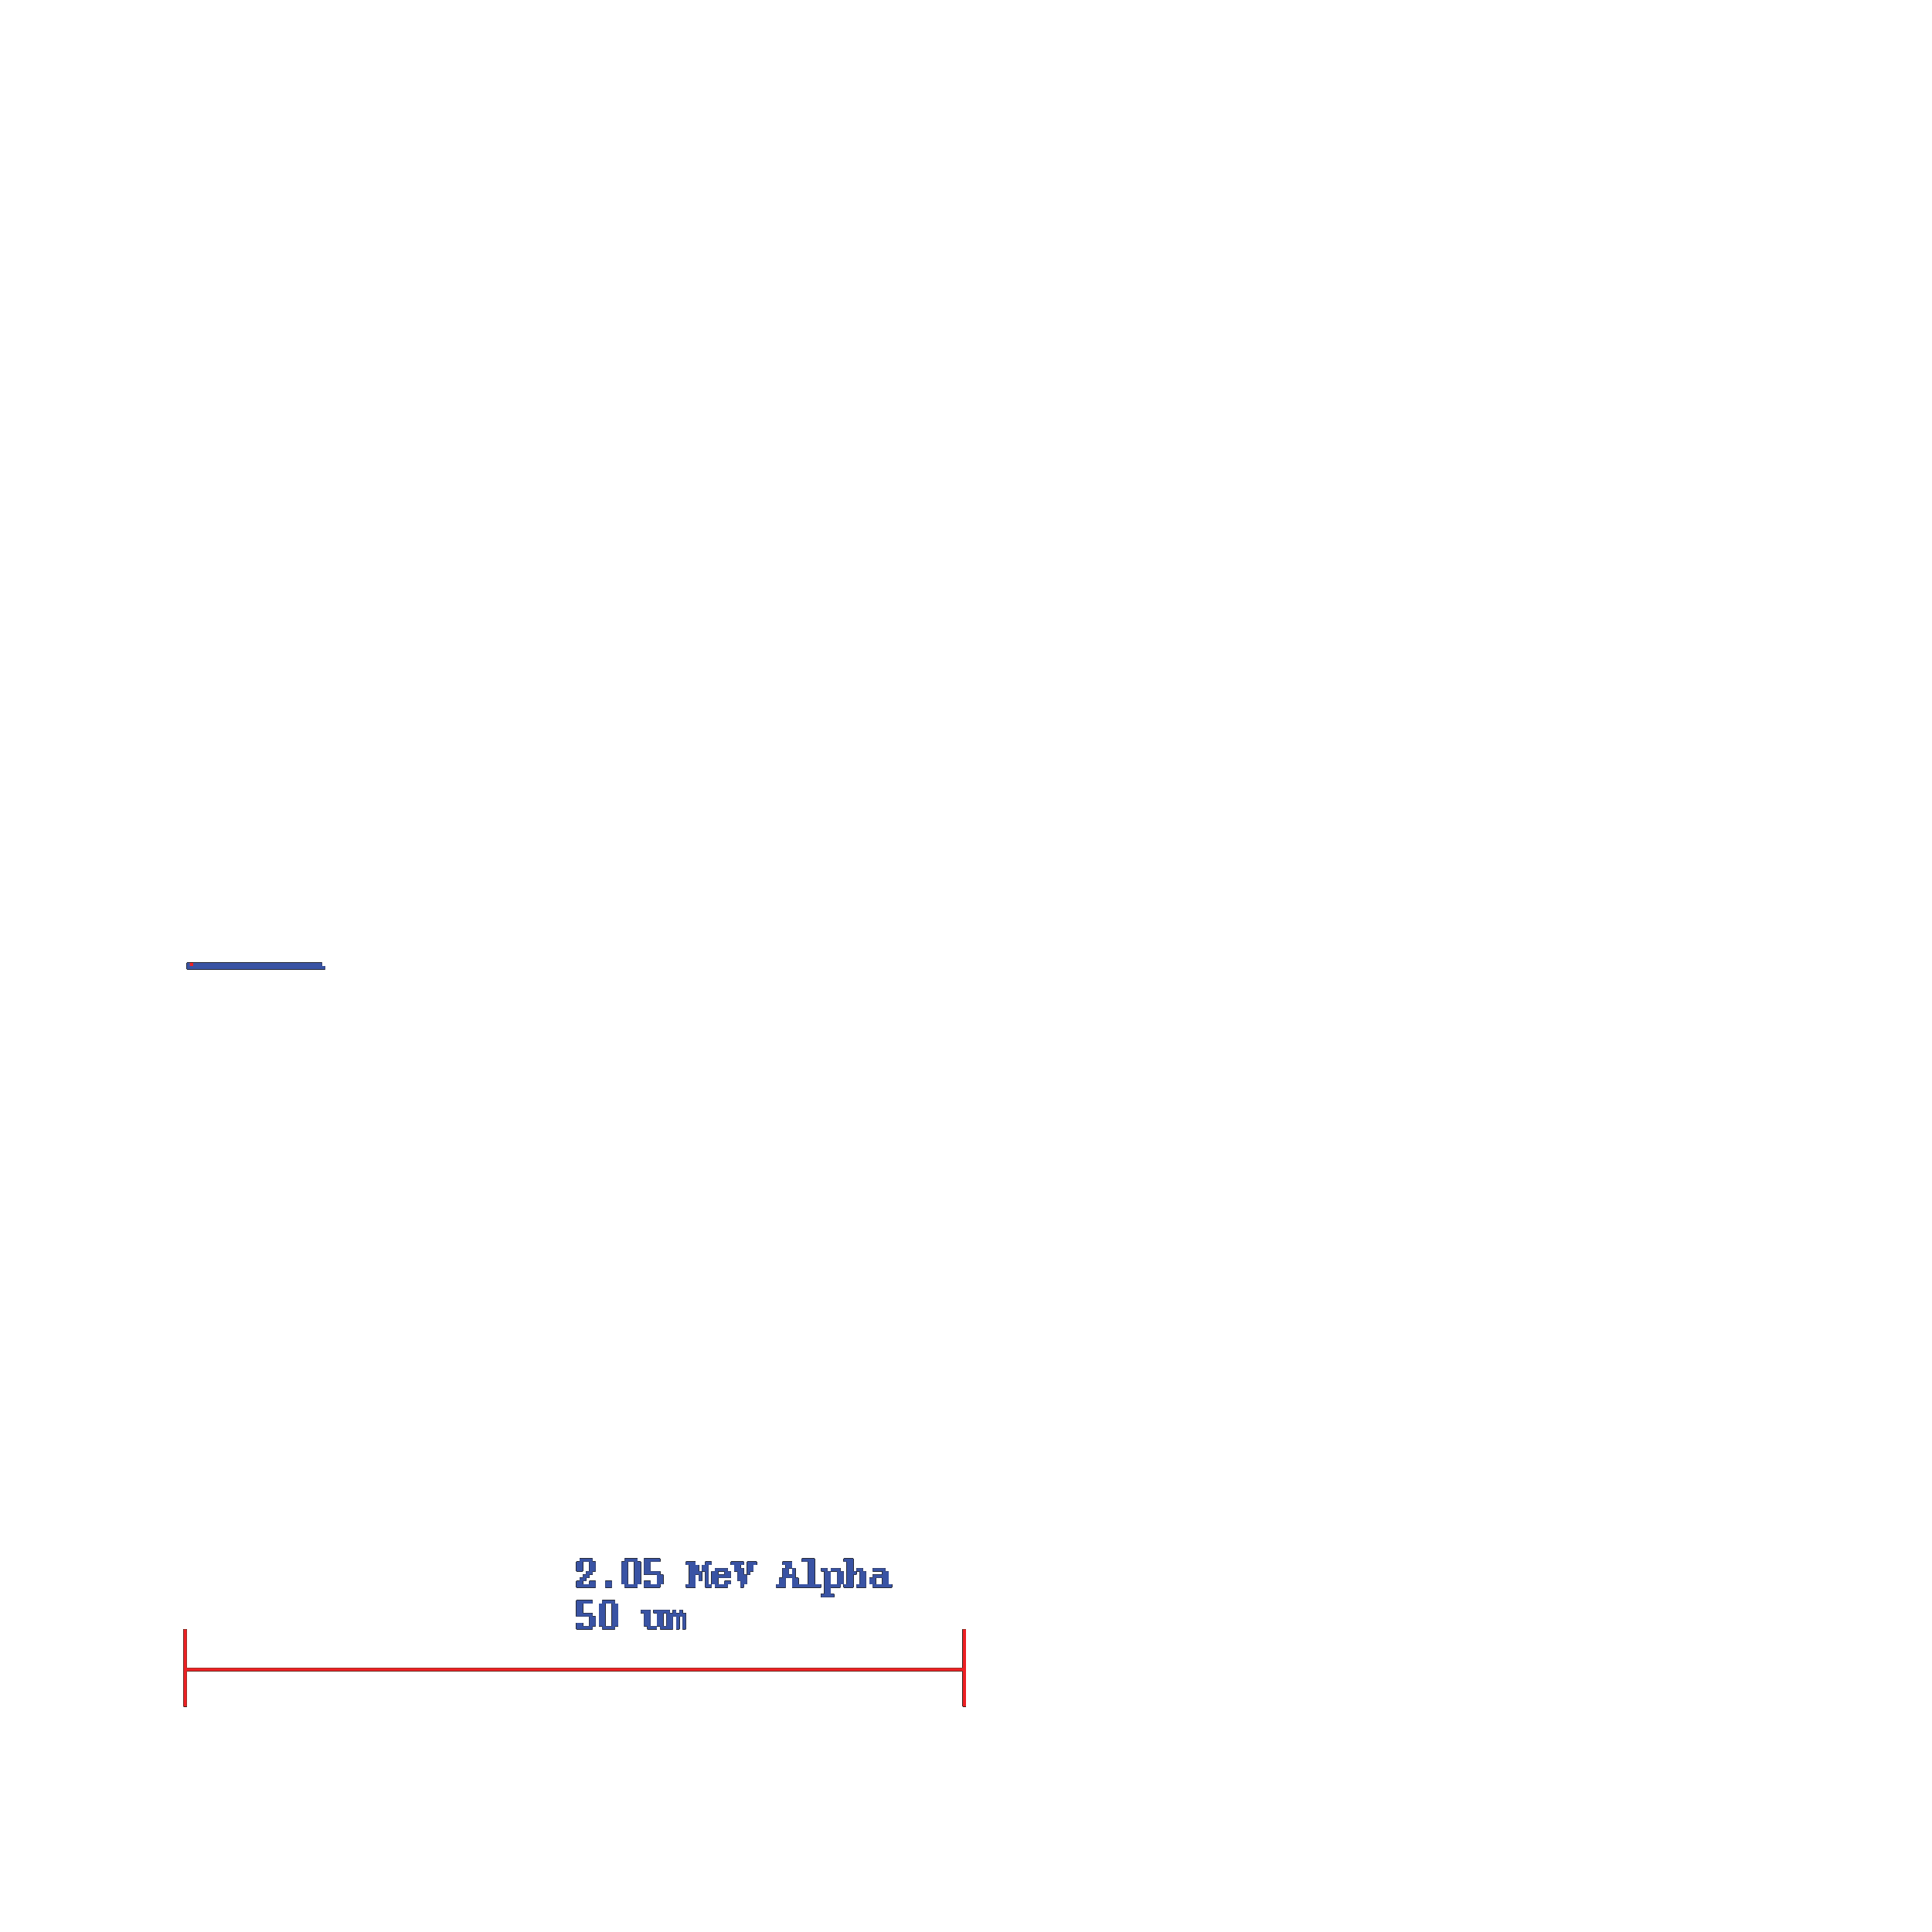
\includegraphics[width=\textwidth]{alphaTrack_0}
    \caption{\SI{2.05}{\MeV} Alpha}
  \end{subfigure}% 
  ~
  \begin{subfigure}[b]{0.45\textwidth}
    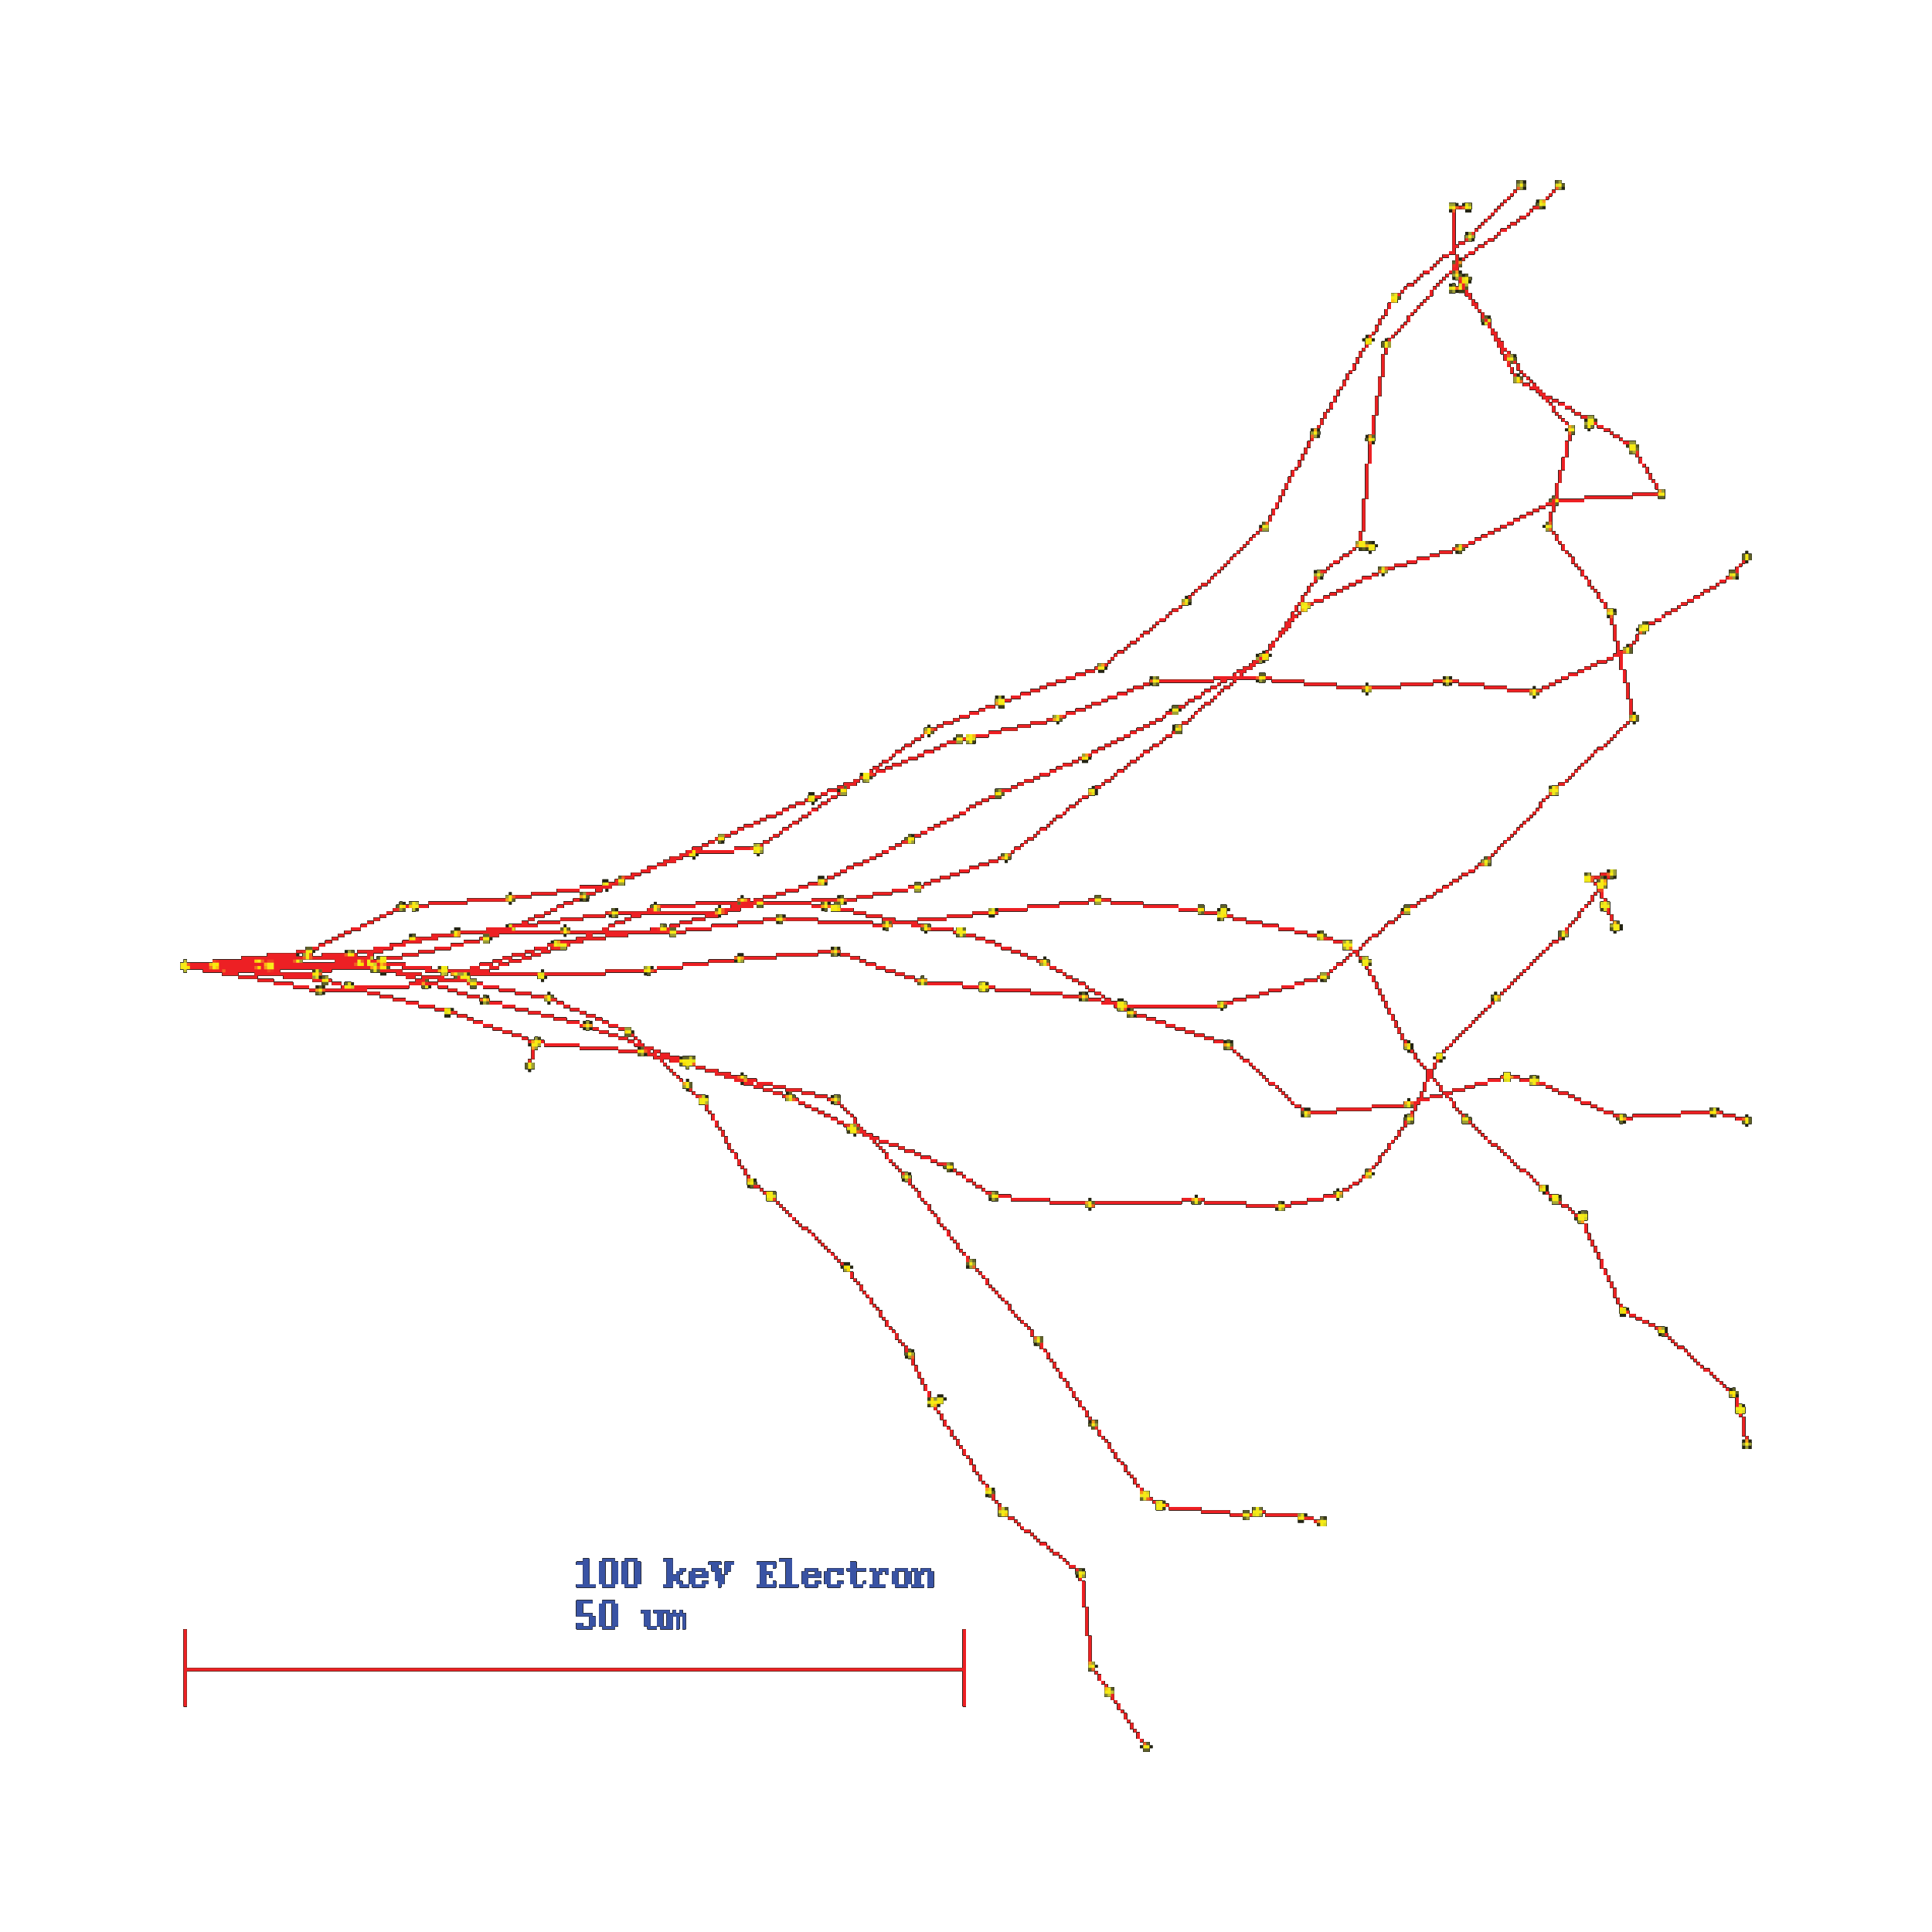
\includegraphics[width=\textwidth]{electronTrack_100keV_0}
    \caption{\SI{100}{\keV} Electron}
  \end{subfigure}
  
  \begin{subfigure}[b]{0.45\textwidth}
    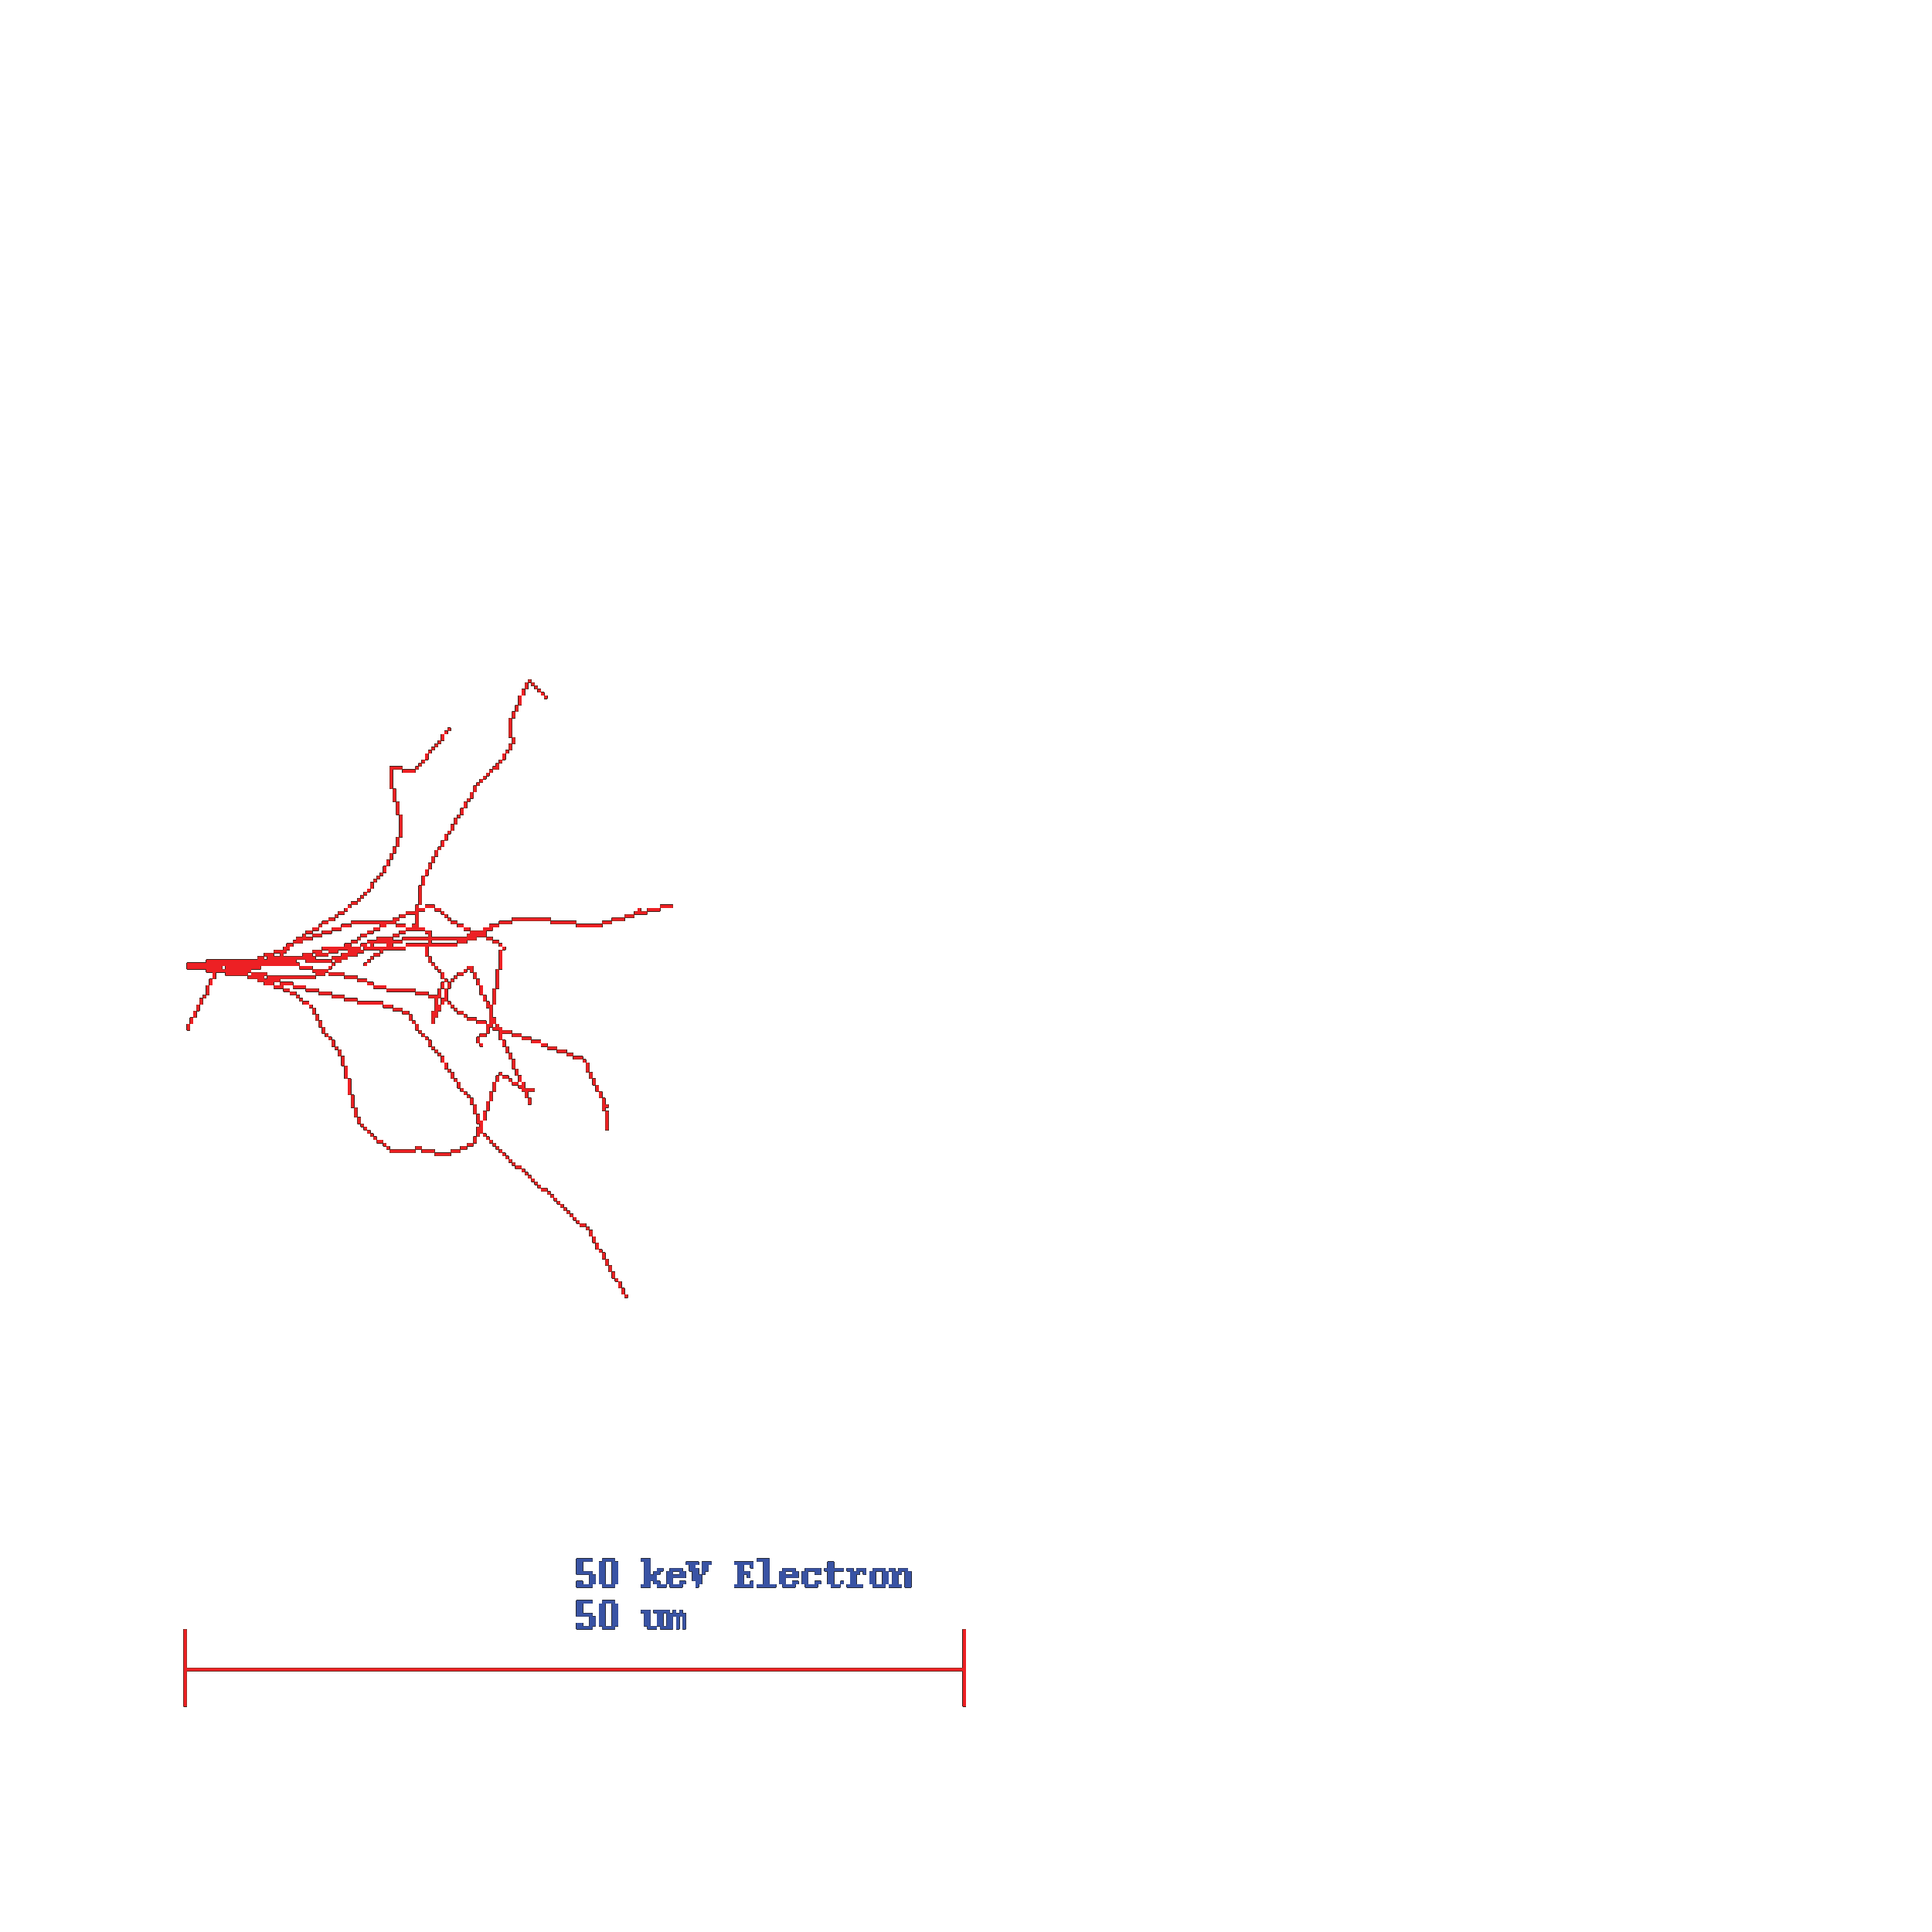
\includegraphics[width=\textwidth]{electronTrack_50keV_0}
    \caption{\SI{50}{\keV} Electron}
  \end{subfigure}%
  ~
  \begin{subfigure}[b]{0.45\textwidth}
    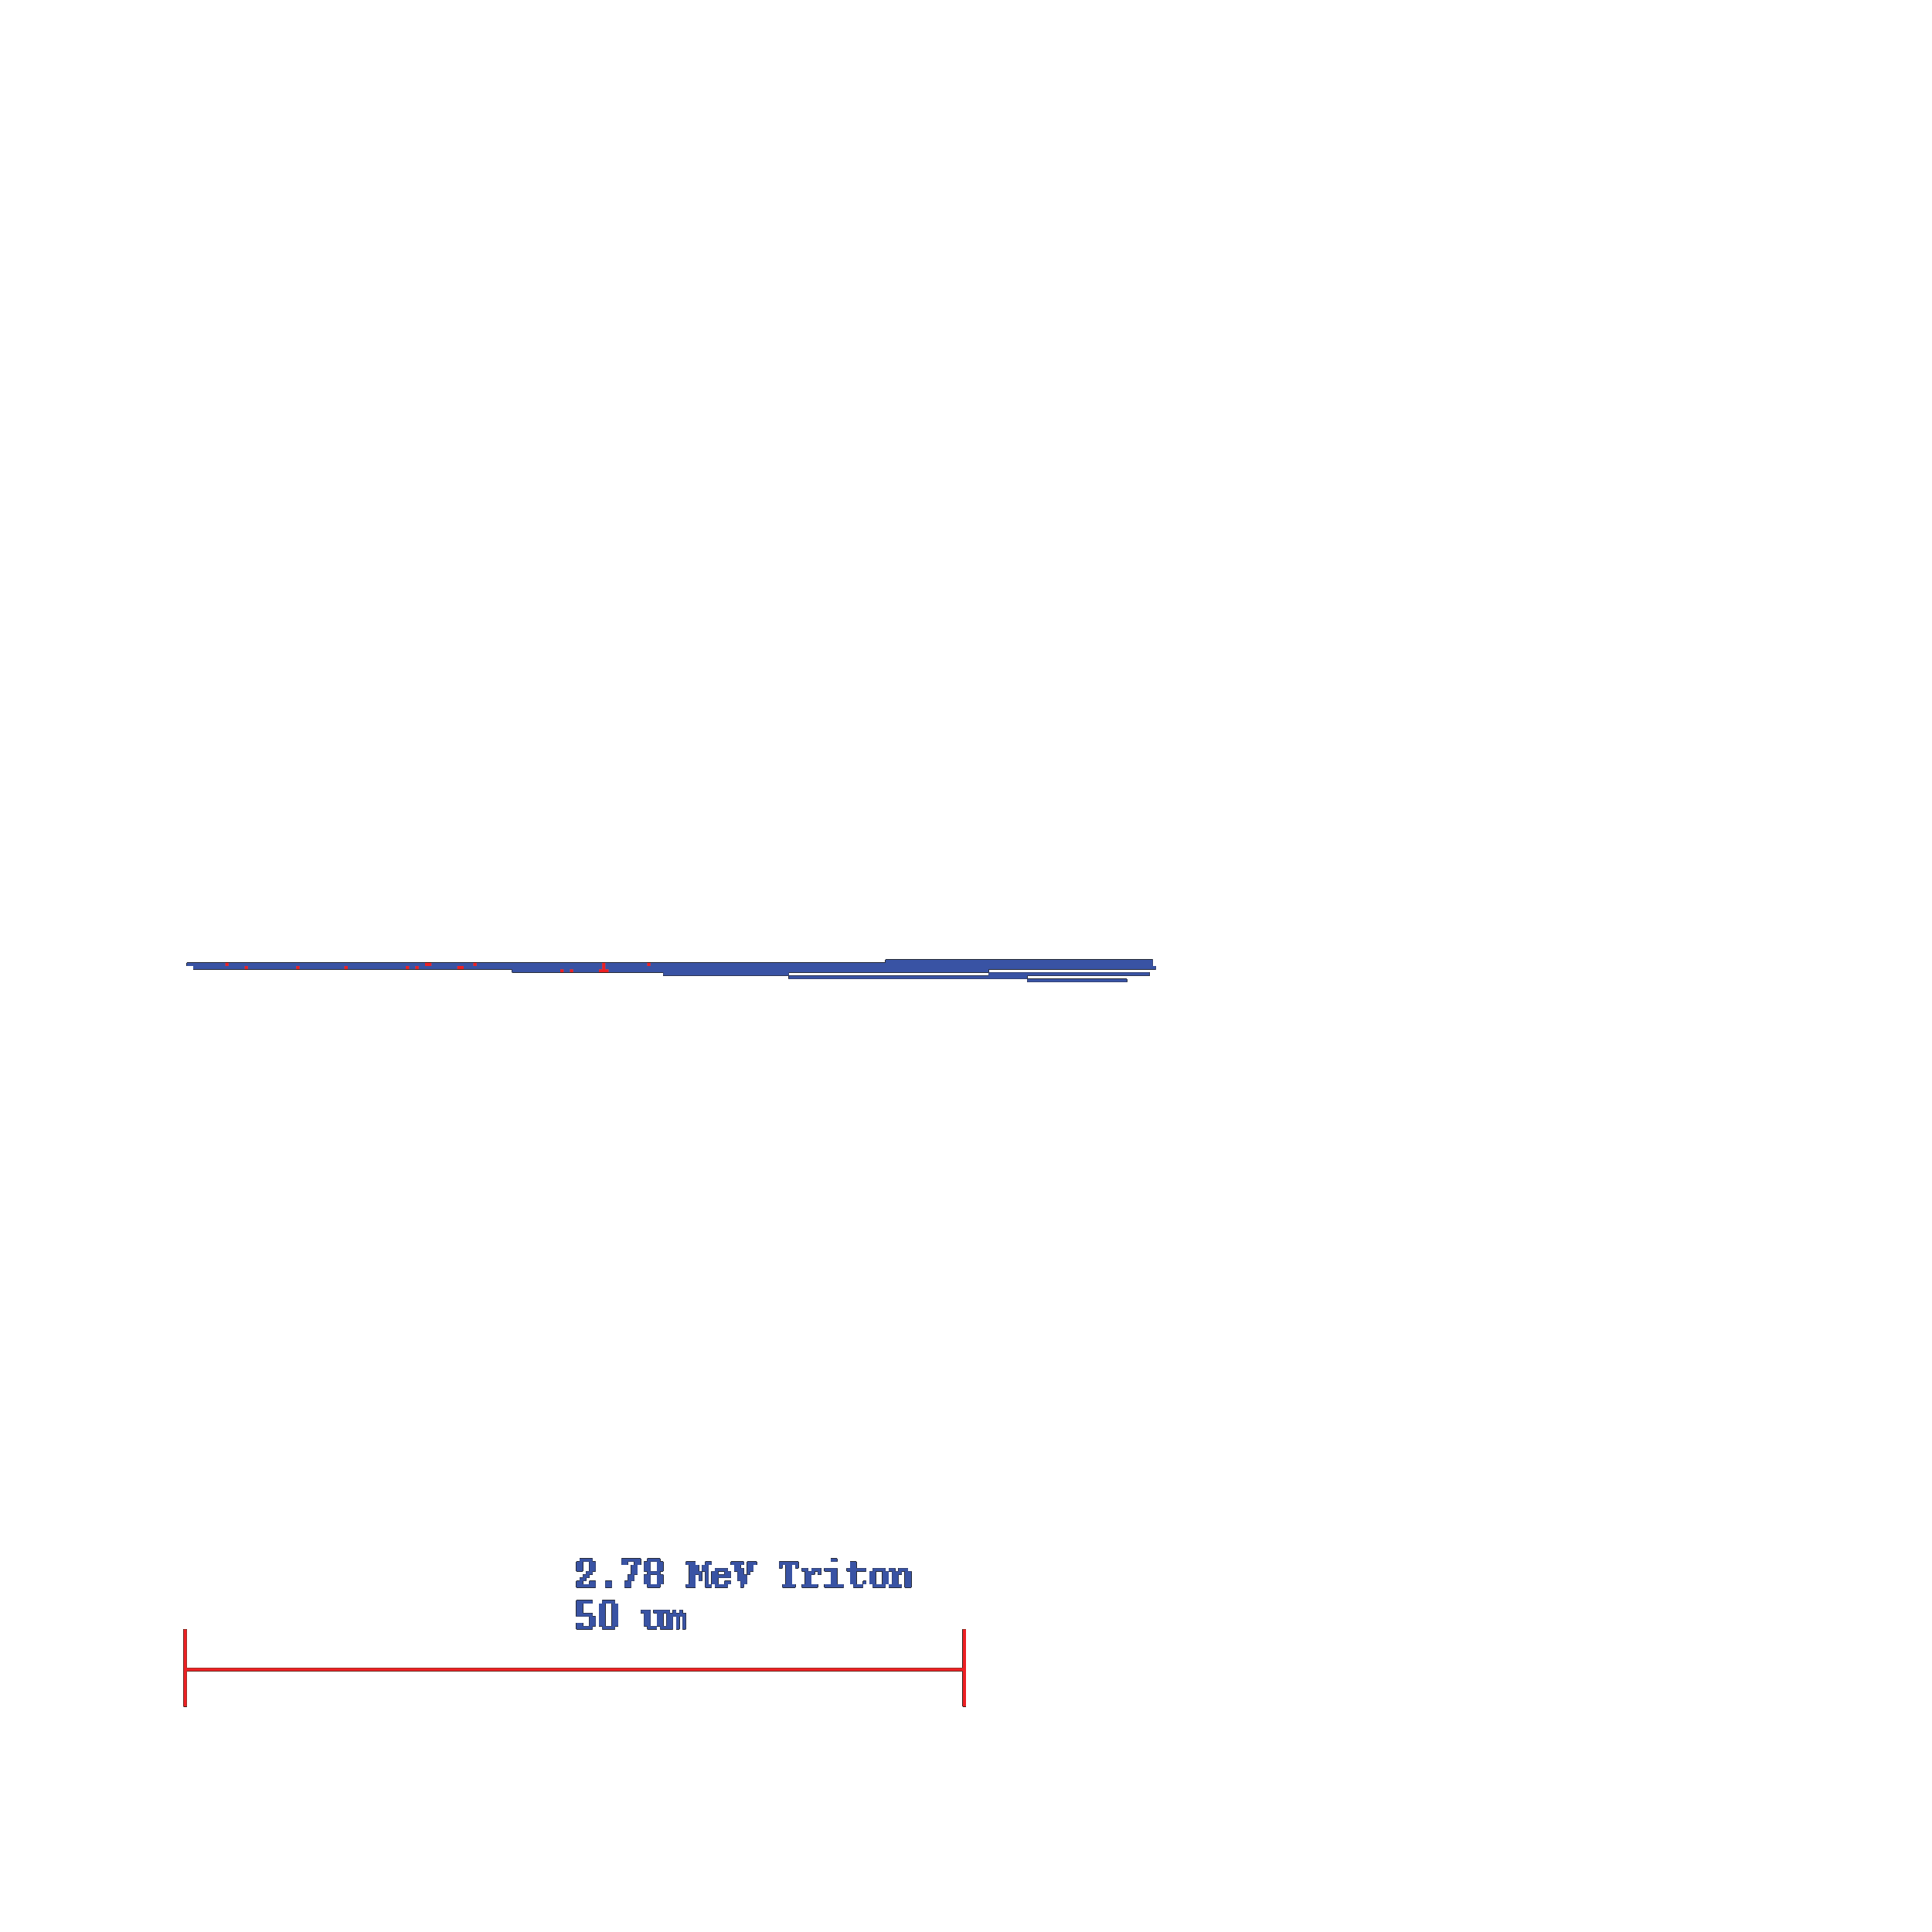
\includegraphics[width=\textwidth]{tritonTrack_0}
    \caption{\SI{2.73}{\MeV} Triton}
  \end{subfigure}
  \caption[Particle Tracks of Alpha, Triton and Electrons]{GEANT4 simulated Particles tracks of a \SI{10}{\keV} electron, \SI{100}{\keV} electron, \SI{2.05}{\MeV} alpha, and \SI{2.73}{\MeV} triton.  The electron tracks are alot broader than the heavy ion tracks, resulting in a greater spread of the energy deposition and less quenching.}
  \label{fig:ParticleTracks}
\end{figure}

For a portal monitor scintillator the most likely charged particles would be alphas, tritons and electrons.
GEANT4 has the capability to simulate light quenching by setting an appropriate Birks parameter, and \autoref{fig:SimLightOutputQuench} presents GEANT4 simulated photon distributions in polystyrene with a PPO-POPOP fluor and an assumed light yield of 1,000 photons per MeV.
For highly energetic particles the electrons are almost an order of magnitude more efficient at creating light than the tritons, and about 90 times more efficient than the alphas, as shown in \autoref{fig:SimNumOP}.
However, it is unlikely that many electrons originating from \iso[60]{Co} interactions in the scintillator will have an energy in the \SI{1}{\MeV} range, more likely that they will be in the \SI{100}{\keV} range.
Thus, as shown in \autoref{fig:SimLightOutputQuench} the triton from the \iso[6]{Li} reaction will produce about an factor of five more photons than an \SI{100}{\keV}, and dominates the number of photons produced the the alpha particle.
\begin{figure}
  \centering
    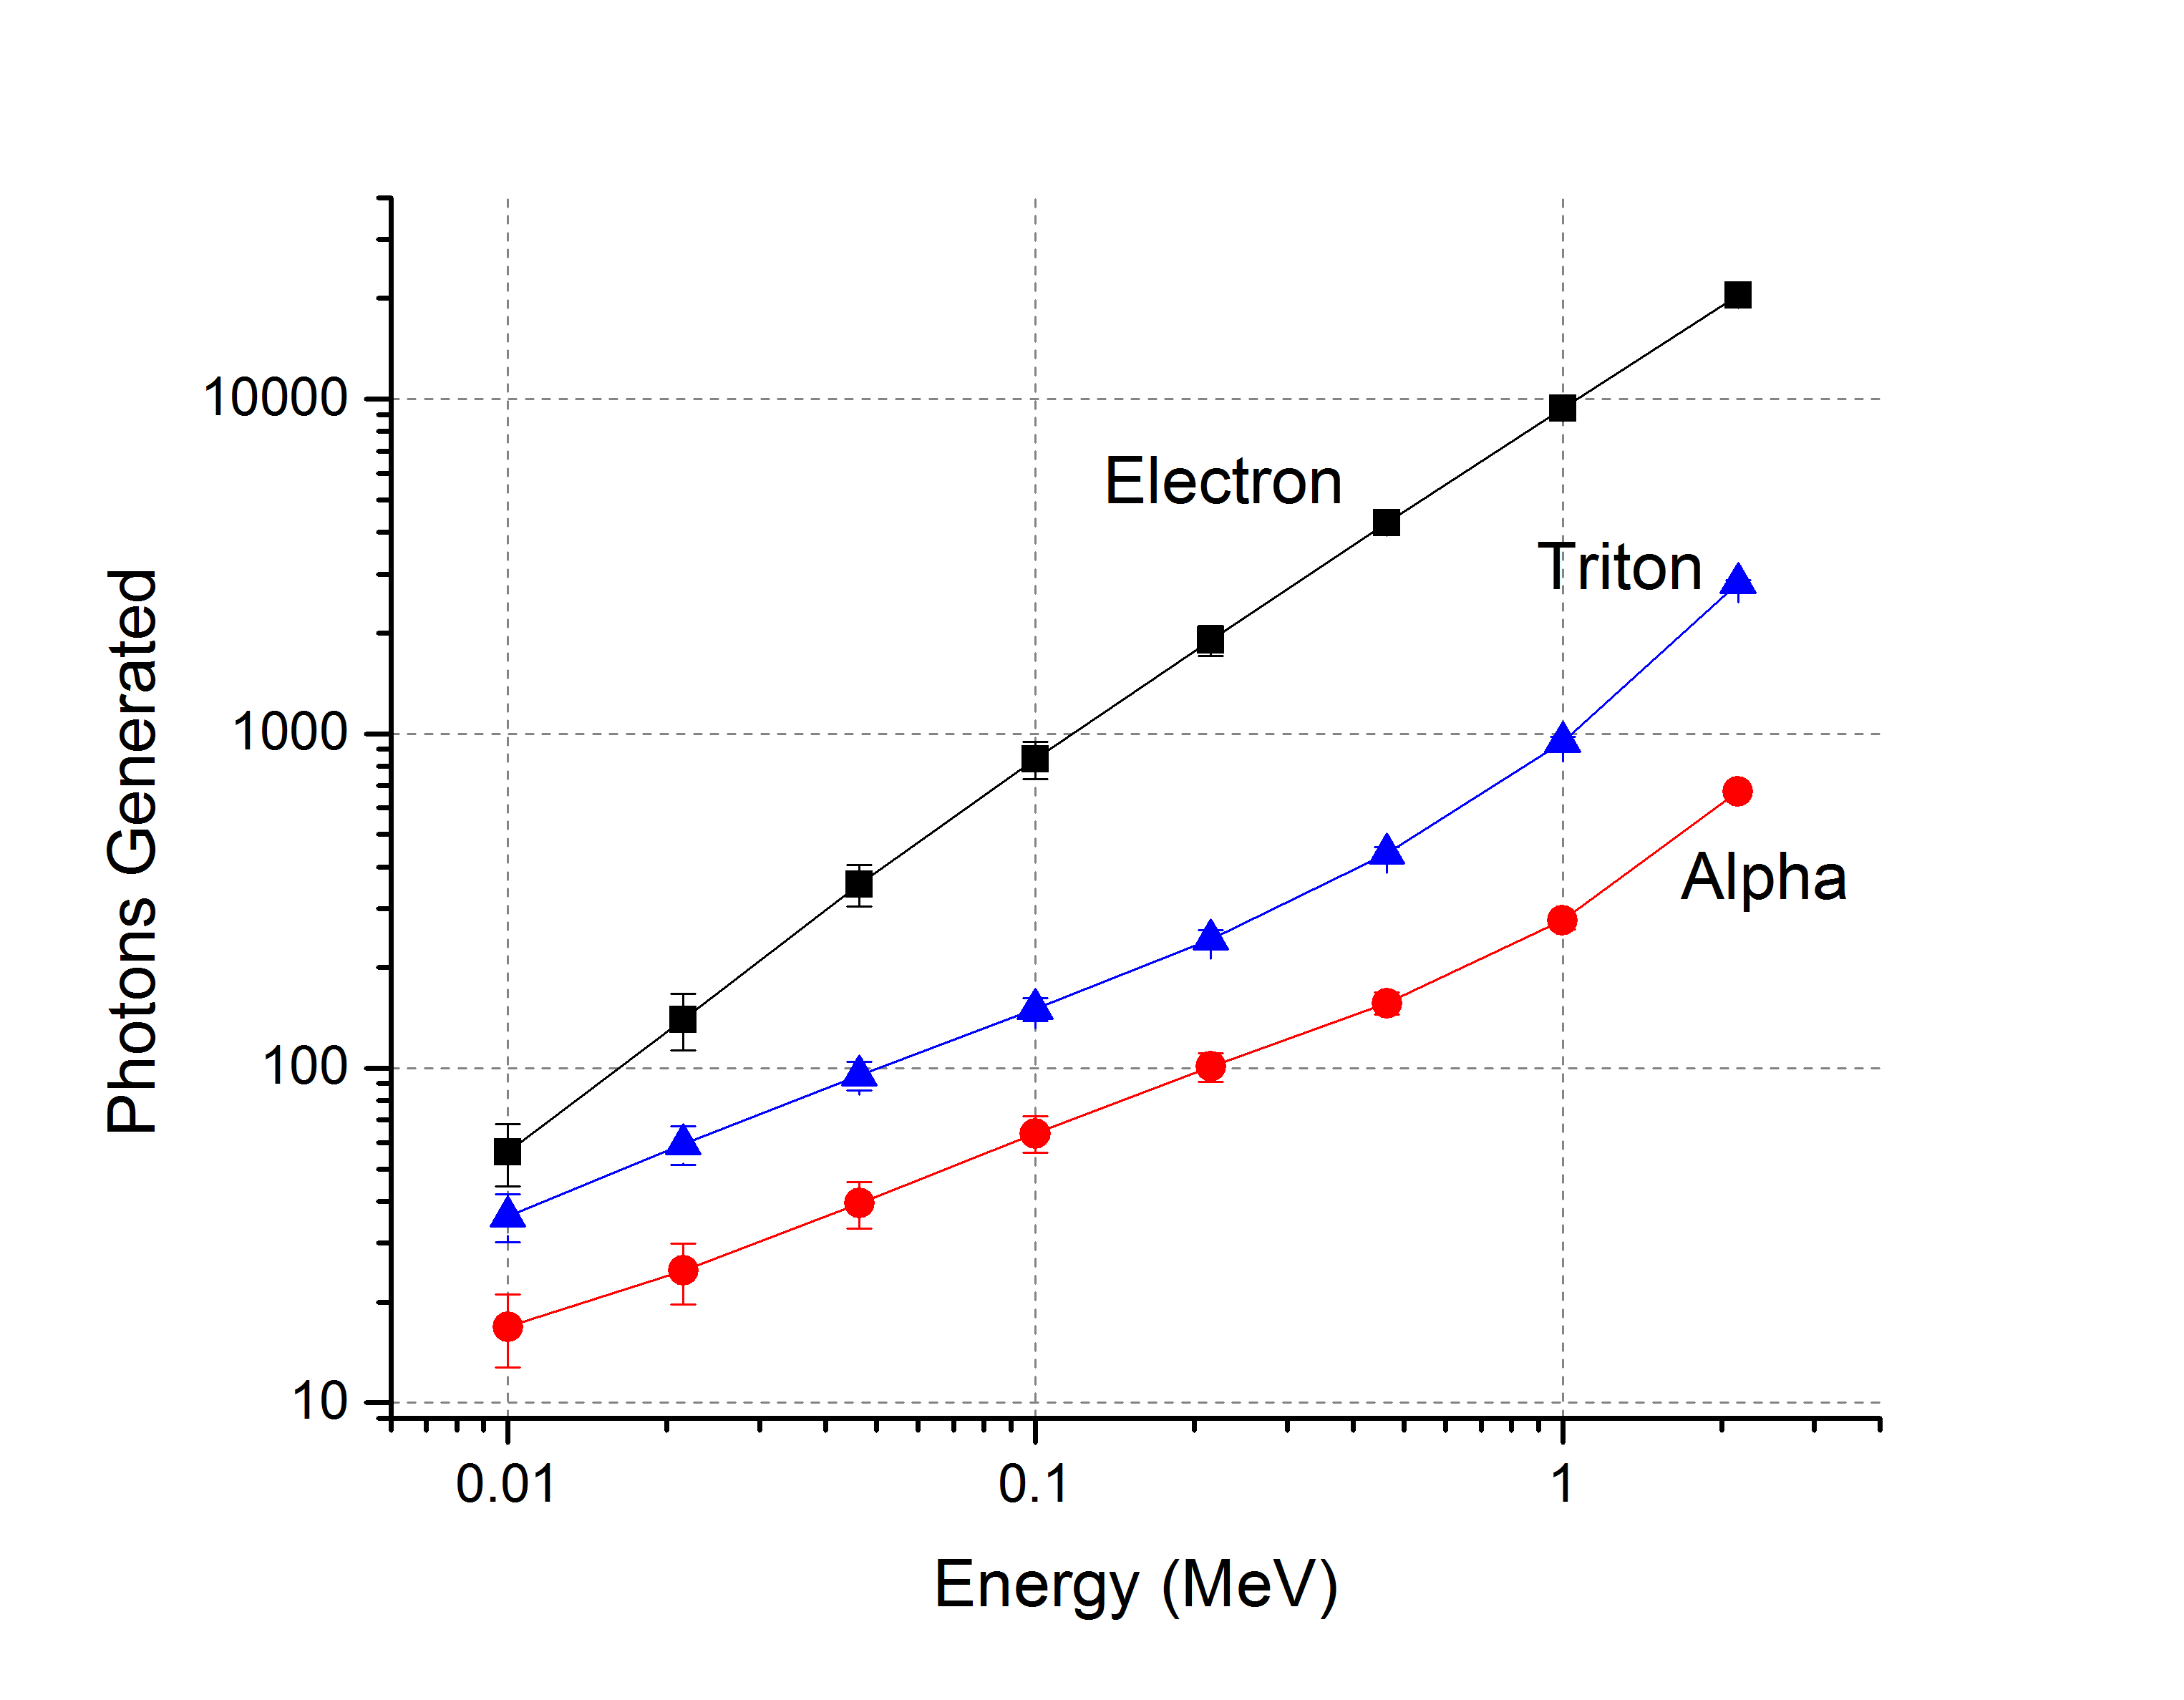
\includegraphics[width=\textwidth]{SimLightQuench}
    \caption[Simulated Number of Optical Photons for Various Ions and Energies]{Simulated number of optical photons generated for electrons, alphas, tritons and \iso[7]{Li}.}
	\label{fig:SimNumOP}
  \end{figure}
  \begin{figure}
	\centering
    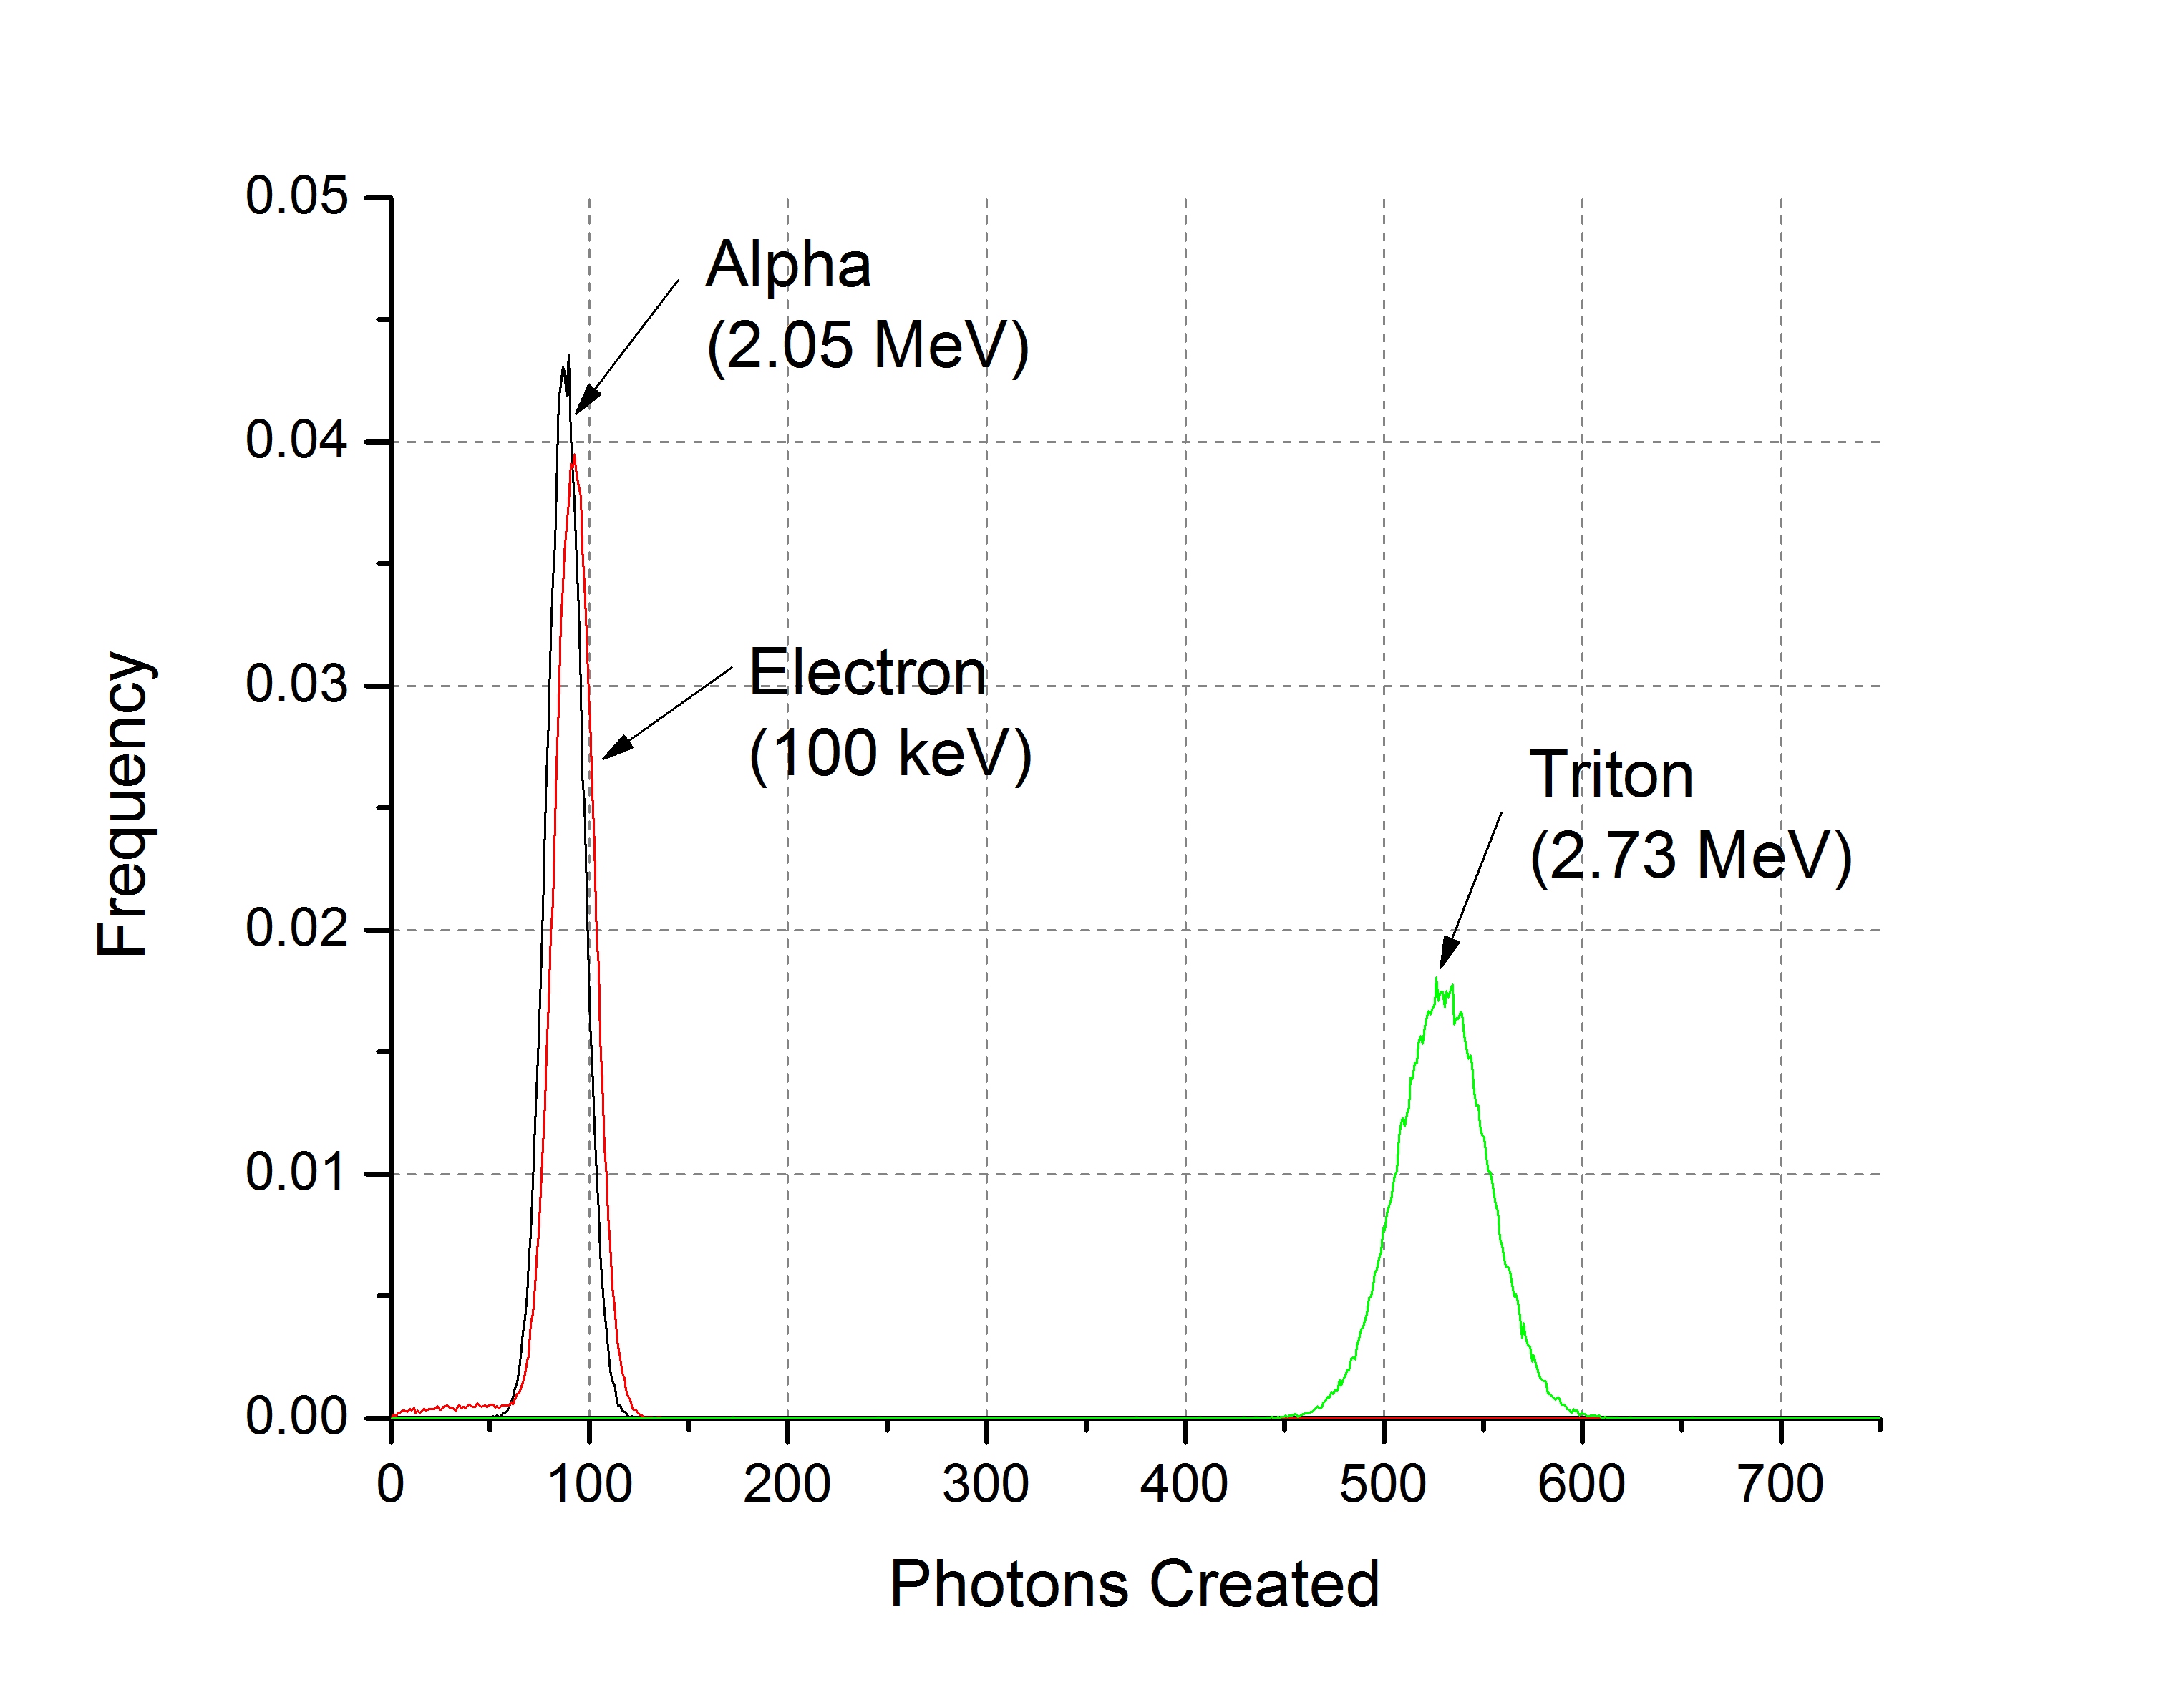
\includegraphics[width=\textwidth]{LightSim_AlphaTritonElectron}
  \caption[GEANT4 simulated light output of alpha, tritons and electrons in polystryene]{Simulated optical photons distributions for the particles of intrest in a portal monitor. The light yield was assumed to be 10,000 photons per MeV.}
  \label{fig:SimLightOutputQuench}
\end{figure}

The pulse height deficit is computed by simulation of the charged particles and the corresponding electron.
This analysis yields a  pulse height deficit for the \iso[6]{Li} reaction as 8.5, and 27 for the \iso[10]{B}.
These results are summarized in \autoref{tab:PulseHeightDeficitSim}.
\begin{table}
  \caption[Simulated Number of Optical Photons for Selected Neutron Absorbitions]{GEANT4 simulated number of optical photons produced for the \iso[10]{B} and \iso[6]{Li} neutron absoribitions.  The sctintillator is assumed to have a light yeild of 1,000 photons per MeV}
  \label{tab:PulseHeightDeficitSim}
  \centering
  \begin{tabular}{c c c | c}
    \toprule
    & Particle & Photons Produced & Pulse Height Deficit \\
    \midrule
    \multirow{3}{*}{\iso[10]{B}} & $\alpha$ (\SI{1.78}{\MeV}) & 72 $\pm$ 8 &  \\
    & \iso[7]{Li} (\SI{1.02}{\MeV}) & 42 $\pm$ 8 & 27 \\
    & electron (\SI{2.78}{\MeV}) & 3,030 $\pm$ 160 & \\
    \hline
    \multirow{3}{*}{\iso[6]{Li}} & $\alpha$ (\SI{2.05}{\MeV}) & 87 $\pm$ 9 & \\
    & triton (\SI{2.75}{\MeV}) & 528 $\pm$ 23 & 8.5\\
    & electron (\SI{4.78}{\MeV}) & 5,250 $\pm$ 300 & \\
    \bottomrule
  \end{tabular}
\end{table}


%%%%%%%%%%%%%%%%%%%%%%%%%%%%%%%%%%%%%%%%%%%%%%%%%%%%%%%%%%%%%%%%%%%%%%%%%%%
%                                                                         %
%                      OPTICS and LIGHT TRANSPORT                            %
%                                                                         %
%%%%%%%%%%%%%%%%%%%%%%%%%%%%%%%%%%%%%%%%%%%%%%%%%%%%%%%%%%%%%%%%%%%%%%%%%%%
\section{Optics and Light Transport}
\label{sec:OpticsTheory}
One would like to collect as much light as emitted from the scintillator as possible.
In practice two effects limit the fraction of the emitted light collected; the optical self-absorption in the material and losses at the edges of the optical surfaces \cite{knoll_radiation_2009}.
The optical self-absorption of a scintillator is a material property in which photons are reabsorbed by the material.
This effect is important for large area scintillators and for scintillators which are not optically  clear, both of which apply to the developed polymeric scintillators.
Typically this effect is mitigated by the use of a wavelength shifting fiber in which the light is transferred to a material which has a much lower optical self-absorption.

Light collection of a scintillation event is emitted isotropically, and therefore only a very small fraction of the photons can travel directly to a photon detector surface.
The majority of the light must then be collected by reflecting back into the medium.
Snell's law governs the reflection of light at an optical boundary, and there are two cases to consider as shown in \autoref{fig:SnellsLaw} and described by Snell's Law, \eqref{eqn:SnellsLaw}
\begin{align}
	\theta_c = \sin^-1 \frac{n_1}{n_0}
	\label{eqn:SnellsLaw}
\end{align}
where \definevar{$\theta_c$}{critical angle}, \definevar{$n_1$}{index of refraction of the surrounding medium} and \definevar{$n_0$}{index of refraction of the scintillator}.
If the angle of incidence, $\theta$, is greater than the critical angle total internal reflection will occur.
When the angle of incidence is less than the critical angle particle reflection (or \textit{Fresnel} reflection) will occur and there will be partial transmission of the photons to the surrounding medium.
\begin{figure}
	\centering
	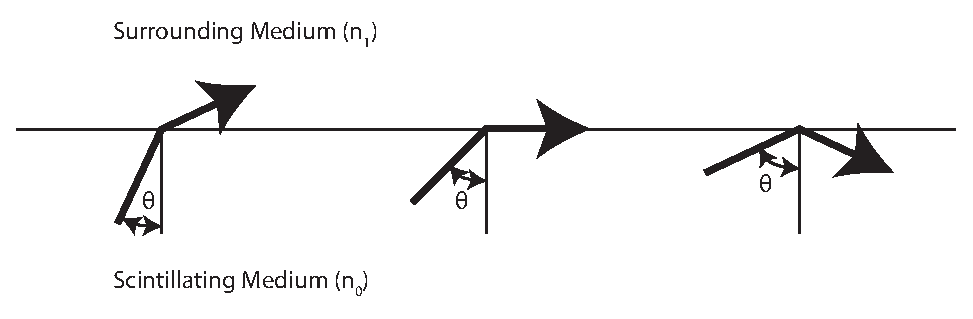
\includegraphics[width=\textwidth]{LightBoundary_SnellsLaw}
	\caption[Light Reflection at a Boundary]{Reflection of light at an optical surface is governed by Snell's law.  The fraction of light reflected back into the material is greatest at an angle of incident equal to $\theta_c$}
	\label{fig:SnellsLaw}
\end{figure}
To ensure that the light stays within the desired medium it is usually encased in a reflector, of which there are two types (\autoref{fig:SpecularDiffusive}).
A polished metallic surface (such as aluminized mylar) may be applied as a specular reflector which are generally better when the length is much longer than the thickness\cite{SaintGobain_DAM_2012}.
A diffusive reflector, such as teflon tape, is better for conditions when the detector is thick compared to its length \cite{knoll_radiation_2009}.
\begin{figure}
	\centering
	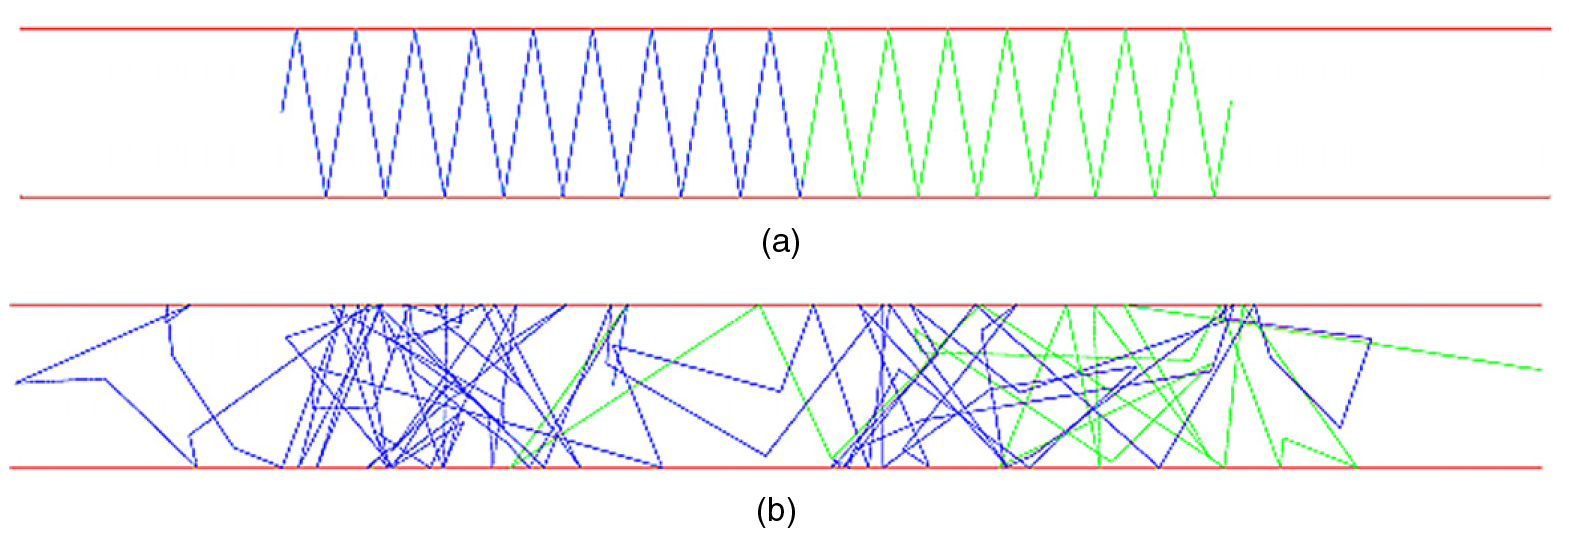
\includegraphics[width=\textwidth]{Riggi_SpecularDiffusive}
	\caption[Specular and Diffusive Reflection]{Specular reflection (a) in which the light in a single incoming direction is emitted as a single outgoing direction. The rough surface of a diffusive reflector (b), causes the light to be reflected at many angles. Figure from \cite{riggi_introducing_2011}.}
	\label{fig:SpecularDiffusive} 
\end{figure}
It should be noted, however, that one would like to optically match the surface at which the scintillator is to be viewed to prevent reflection.

Photons that are emitted exactly along the direction of the scintillator will only be effected by the  absorption length of the material (typically on the order of \SI{100}{\cm} to \SI{400}{\cm} \cite{SG_PlasticScint_2008}) while photons emitted in directions nearly normal to the direction of the scintillator will need to undergo thousands of reflections in order reach the PMT, which can double the length the photons must travel.
For perfect specular reflection it has been shown through simulation the the number of photons throughout a scintillating strip is only reduced by the optical absorption in that strip \cite{riggi_introducing_2011}.
In a realistic scintillator with a diffusive reflector the number of photons decreases by a factor of more than 10 \SI{50}{\cm} from the origination of the photon\cite{riggi_introducing_2011}.

In the cases of a large scintillating detector, such as the one presented in this work, it  may be necessary to employ more than one PMT to collect the light.
In such cases the use of light pipes may enhance the collection efficiency. 
Light pipes are not without costs, however, as they are generally of a high index of refraction to maintain a high internal reflection
